


\listfiles

\documentclass[	hyperref={pdfpagelabels=false}, xcolor=dvipsnames,
		11pt]{beamer}

% 
\newcommand*{\PTAS}{PTAS}

\newcommand*{\IE}{i.e.}
\newcommand*{\EG}{e.g.}

\newcommand*{\keyword}[1]{\emph{#1}\index{#1}}
% \newcommand*{\comments}[1]{}

\newcommand{\CORR}{\mathrel{\widehat{=}}}

\newcommand*{\SU}[1]{SU(#1)}
% \newcommand*{\Z}[1]{Z(#1)}
\newcommand*{\Z}[1]{\mathbb{Z}_{#1}}

\newcommand*{\DIM}[1]{#1-dimensional}
\newcommand*{\COMMA}{\quad ,}
\newcommand*{\POINT}{\quad .}
\newcommand*{\MEAS}[1]{\mathcal{D}[#1]}


\DeclareMathOperator{\Tr}{tr}
\DeclareMathOperator{\e}{e}

\newcommand*{\tr}[1]{\Tr \ [ \ #1 \ ]}

\newcommand*{\FIG}[1]{Figure~\ref{#1}}
\newcommand*{\FIGs}[2]{Figures~\ref{#1} - \ref{#2}}
\newcommand*{\TAB}[1]{Table~\ref{#1}}
\newcommand*{\SEC}[1]{Section~\ref{#1}}
\newcommand*{\CHAP}[1]{Chapter~\ref{#1}}
\newcommand*{\LIST}[1]{Listing~\ref{#1}}
\newcommand*{\PROC}[1]{Procedure~\ref{#1}}
\newcommand*{\EXP}[1]{\langle #1 \rangle}
\newcommand*{\EQU}[1]{Equation~\eqref{#1}}
\newcommand*{\EQUs}[2]{Equations~(\ref{#1}) - (\ref{#2})}
\newcommand*{\APP}[1]{Appendix~\ref{#1}}

%\newcommand{\tr}[1]{\mbox{tr}~\left[#1]}

\renewcommand\Re{\operatorname{Re}}
\renewcommand\Im{\operatorname{Im}}




\newcommand*{\SYM}[1]{\mathcal{#1}}

\newcommand*{\FIGURE}[1]{\textcolor{blue}{Fig.:}}
% \newcommand*{\FIGURE}[1]{}

%  \newcommand{\testbox}[1]{\framebox{#1}}
\newcommand{\testbox}[1]{#1}

\setlength{\fboxsep}{0.0pt}	%	separation between boxes.
\setlength{\fboxrule}{0.05pt}	%	line width of boxes

\newlength{\plotwidth}
\setlength{\plotwidth}{360pt}

\newlength{\testwidth}
\setlength{\testwidth}{0.25\textwidth}
 
\setlength{\unitlength}{0.95\textwidth}  % measure in textwidths


\newlength{\one}
\setlength{\one}{0.85\textwidth}

\newlength{\onehalf}
\setlength{\onehalf}{0.51\textwidth}

\newlength{\onethird}
\setlength{\onethird}{0.31\textwidth}

\newlength{\twofifth}
\setlength{\twofifth}{0.35\textwidth}


% \def\dblone{\hbox{$1\hskip -1.2pt\vrule depth 0pt height 1.6ex width 0.7pt\vrule depth 0pt height 0.3pt width 0.12em$}}

%     \setbeamerfont{section title}{parent=title}
%     \setbeamercolor{section title}{parent=titlelike}
%     \defbeamertemplate*{section page}{default}[1][]
%     {
%       \centering
%         \begin{beamercolorbox}[sep=8pt,center,#1]{section title}
%           \usebeamerfont{section title}\insertsection\par
%         \end{beamercolorbox}
%     }
%     \newcommand*{\sectionpage}{\usebeamertemplate*{section page}}

\definecolor{arrowred}{RGB}{255,105,105}
\definecolor{arrowblue}{RGB}{105,105,255}
\definecolor{resultgreen}{RGB}{246,255,213}
\definecolor{resultgreenedge}{RGB}{0,128,0}


\AtBeginSection[]{
  \begin{frame}
  \vfill
  \centering
  \begin{beamercolorbox}[sep=8pt,center,shadow=true,rounded=true]{title}
    \usebeamerfont{title}\insertsectionhead\par%
  \end{beamercolorbox}
  \vfill
  \end{frame}
}

% 


\usepackage{etex}			% needed to resolve conflicts between booktabs and tikz
\usepackage{tikz}
\usepackage{verbatim}
\usetikzlibrary{arrows,shapes}

 %\usetheme{boxes}
% \usecolortheme{lily}
 %\usecolortheme{rose}

 \usefonttheme{serif}

\usepackage{lmodern}
 \usepackage{graphicx}
 \usepackage{multirow}				%enables multirow tables

\usepackage{natbib}
\bibpunct{[}{]}{,}

\usepackage{epsfig}
\usepackage{layout}

\usepackage{booktabs}

\setbeamercovered{transparent}
\mode<presentation>





 
\beamertemplatenavigationsymbolsempty %Navigationszeile auf jeder Folie unterdrücken






\usepackage{ae,aecompl}				% fuer besseres pdf empfohlen
%\usepackage{exscale}				% richtige Skalierung der Mathe Formeln. Does not work with tikz




\usepackage[mathcal]{euscript}
\usepackage{amsthm}				% adds theorems and lemmata



\usepackage{dsfont}

% \usepackage{fancyhdr}	


% 
% %******************************************************************************
% %
% % Fancyheaders
% %
% \usepackage{fancyhdr}					% Pagehead
% \pagestyle{fancy}					% meine Kopfzeile
% \fancyhf{}
% % \fancyhead[RO]{\rm \nouppercase  \rightmark \qquad \rm \thepage }
% % \fancyhead[LE]{  \thepage  \qquad \rm \nouppercase  \leftmark }
% \fancyhead[RO]{\nouppercase  \rightmark}
% \fancyhead[LE]{ \nouppercase  \leftmark }
% 
% \fancyfoot[OR]{  \thepage}
% \fancyfoot[EL]{ \thepage }
% 
% % \renewcommand{\headrulewidth}{0.1pt}
% 
% \renewcommand{\chaptermark}[1]{\markboth{\thechapter.\ #1}{}}
% 
% 
% \renewcommand{\sectionmark}[1]{\markright{\thesection.\ #1}}
% 
% 
% \fancypagestyle{plain}{%
% \fancyhf{} % clear all header and footer fields
% \fancyfoot[RO,RE]{\thepage} %RO=right odd, RE=right even
% \renewcommand{\headrulewidth}{0pt}
% \renewcommand{\footrulewidth}{0pt}}
% 
% 
% 
% %
% %******************************************************************************






\usepackage{array}		%for readjusting the hight of lines in tables
% \usepackage{longtable}

\usepackage[german,english]{babel}
\usepackage{hyperref}
\hypersetup{colorlinks=false}
%
\DeclareGraphicsExtensions{.eps, .jpg, .png, .sgv, .jepg}
% \usepackage[subsection]{algorithm}
% \usepackage{algorithmic,algorithmic-fix}
\usepackage{listings}
\lstset{ %
language=C++,                   % the language of the code
basicstyle=\footnotesize,       % the size of the fonts that are used for the code
numbers=left,                   % where to put the line-numbers
numberstyle=\footnotesize,      % the size of the fonts that are used for the line-numbers
stepnumber=1,                   % the step between two line-numbers. If it's 1, each line 
                                % will be numbered
numbersep=5pt,                  % how far the line-numbers are from the code
% showspaces=false,               % show spaces adding particular underscores
% showstringspaces=false,         % underline spaces within strings
showtabs=false,                 % show tabs within strings adding particular underscores
frame=bottomline,                   % adds a frame around the code
% tabsize=2,                      % sets default tabsize to 2 spaces
captionpos=t,                   % sets the caption-position to bottom
% breaklines=false,                % sets automatic line breaking
% breakatwhitespace=false,        % sets if automatic breaks should only happen at whitespace
% title=\lstname,                 % show the filename of files included with \lstinputlisting;
                                % also try caption instead of title
% escapeinside={\%*}{*)},         % if you want to add a comment within your code
% morekeywords={*,...}            % if you want to add more keywords to the set
}


\usepackage{caption}
\DeclareCaptionFont{white}{\color{white}}
\DeclareCaptionFormat{listing}{\colorbox{gray}{\parbox{\textwidth}{#1#2#3}}}
\captionsetup[lstlisting]{format=listing,labelfont=white,textfont=white}











\usepackage{parskip}		%kills the default paragraph indenting and sets /parskip to some useful value automatically



\usepackage{amssymb}
\usepackage{amsmath}
% \usepackage{bbold}
% \usepackage{dsfont}

%Graphics and Videos




%Graphics and Videos

% \usepackage{movie15}






\usepackage{thesisstyle}
\usepackage{thesiscommands}

\logo{
	\raisebox{-.4\height}{
\includegraphics[width=1cm]{./pics/unilogo}} \quad\insertframenumber\quad\quad
}


\title{Preliminaries for Distributed Natural Computing Inspired by the Slime Mold Physarum Polycephalum}
\author{Michael T.\ Dirnberger}
\institute{Max Planck Institute for Informatics}

\date{PhD Defense, 31.07.2017, Saarbr\"ucken\\[2em]}


\begin{document}

\begin{frame}[plain]

\titlepage
\vspace{-1cm}
	    \begin{center}
		
\includegraphics[width=0.3\linewidth]{./pics/mpilogo}
	    \end{center}
\end{frame} 

% 4 slides
\section{Part I: Natural Computing with P.~polycephalum}

\begin{frame}
    \frametitle{Natural Computing in a Nutshell} 

	\begin{columns}
	\begin{column}{5cm}

	\begin{overprint}

		\begin{block}{}
		  \begin{itemize}
		   \item<2-> Design novel nature-inspired algorithms.
		   \item<3-> Synthesize natural phenomena using computers.
		   \item<4-> Use natural materials to do computations.
		  \end{itemize}
		\end{block}

	\end{overprint}

	\end{column}

	\begin{column}{5cm}
	\begin{overprint}

	\testbox{
	\begin{minipage}[t]{5 cm}

	\begin{figure}[h]
		\captionsetup[subfloat]{position=bottom,labelformat=empty,font=scriptsize}
		\begin{center}
			\only<1>{\subfloat[\textcolor{gray}{Wikipedia CC BY-SA 4.0}]{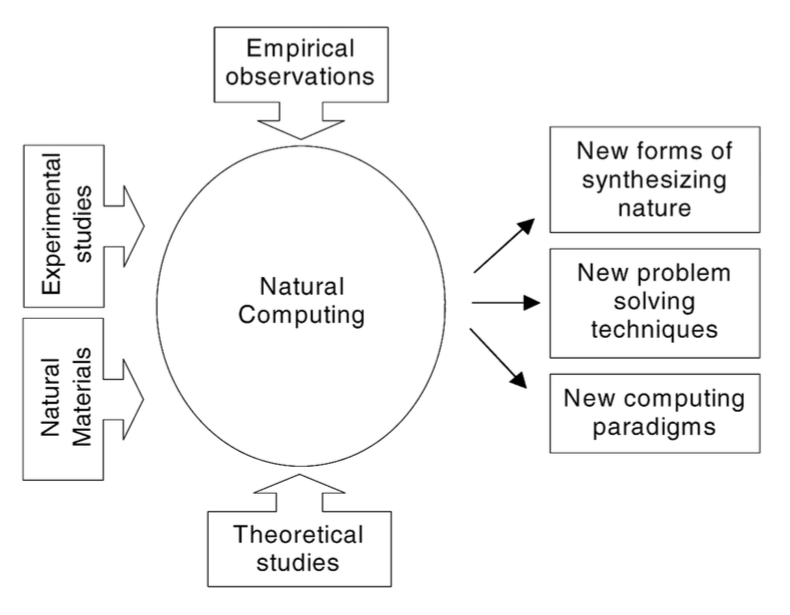
\includegraphics[angle=0,clip=true,width= \linewidth, trim = 0 0 0 0]{./pics/natural_computing.png}}}
			\only<2>{\subfloat[{Ant Colony Optimization, M. Dorigo, 2004}]{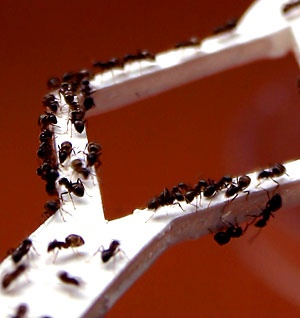
\includegraphics[angle=0,clip=true,width= 0.7\linewidth, trim = 0 0 0 0]{./pics/ants2.jpg}}}
			\only<3>{\subfloat[\textcolor{gray}{Wikipedia CC BY-SA 4.0}]{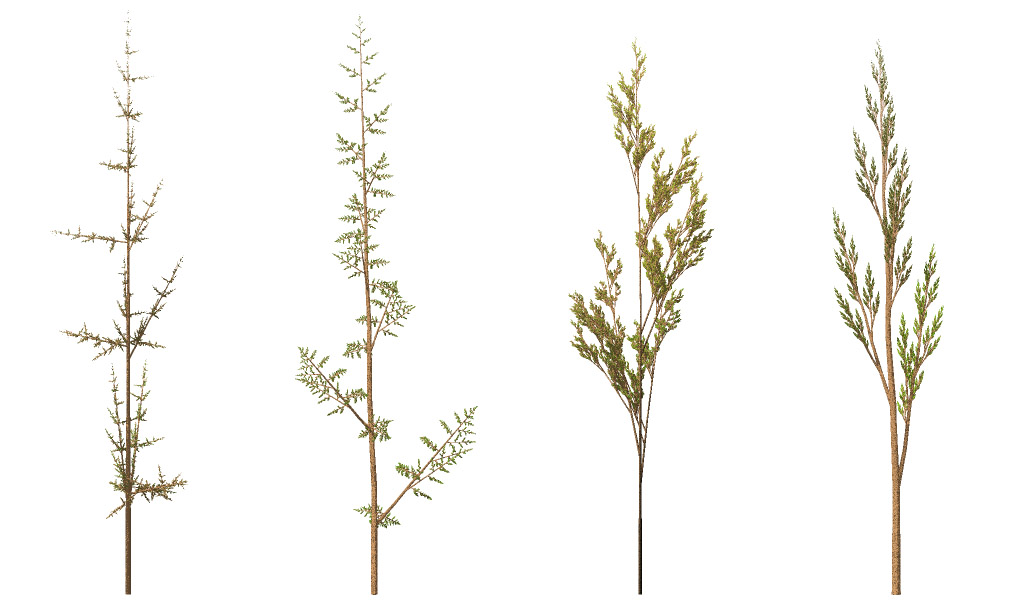
\includegraphics[angle=0,clip=true,width= \linewidth, trim = 0 0 0 0]{./pics/weeds.jpg}}}
			\only<4>{\subfloat[\textcolor{gray}{Wikipedia CC BY-SA 4.0}]{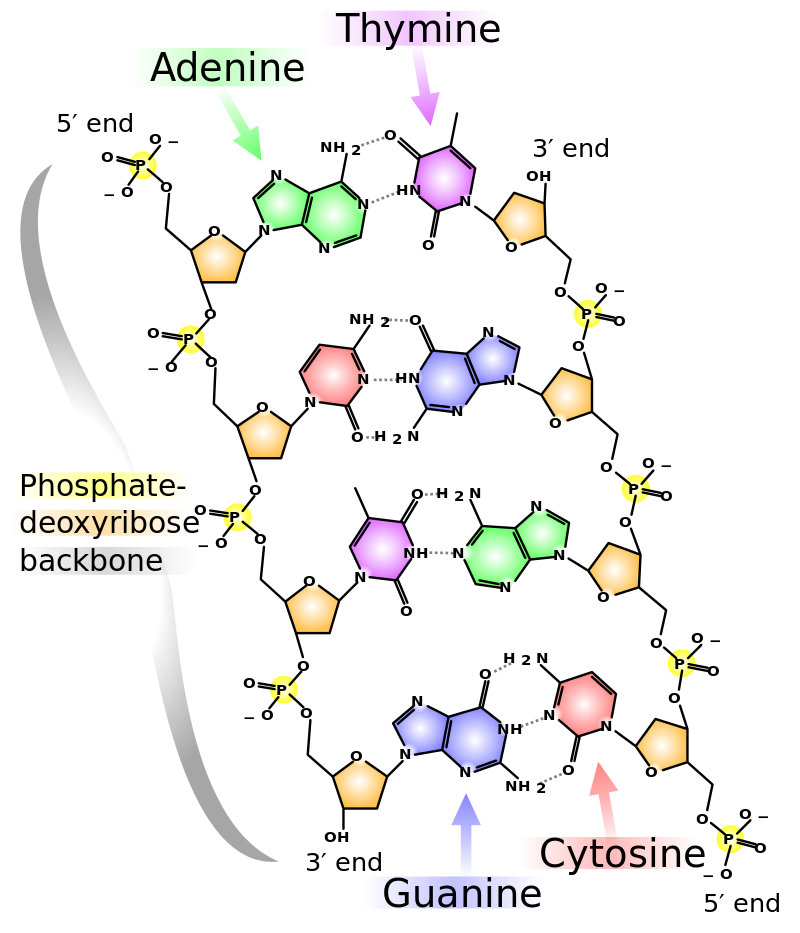
\includegraphics[angle=0,clip=true,width= 0.67\linewidth, trim = 0 0 0 0]{./pics/dna.png}}}
		\end{center}
	\end{figure}
	\end{minipage} }

	\end{overprint}
	\end{column}
	\end{columns}

	\begin{center}
		\textcolor{red}{Natural Computing is a highly interdisciplinary field!}
	\end{center}
\end{frame}

\begin{frame}
    \frametitle{A Magnificent Mold} 

	\begin{columns}
	\begin{column}{5cm}

	\begin{overprint}

		\begin{block}{\Pp:}
		  \begin{itemize}
		   \item<2-> Unicellular organism with many nuclei.
		   \item<3-> Intricate foraging strategy.
		   \item<4-> Networks circulate protoplasm.
		  \end{itemize}
		\end{block}

	\end{overprint}

	\end{column}

	\begin{column}{5cm}
	\begin{overprint}

	\testbox{
	\begin{minipage}[t]{5 cm}

	\begin{figure}[h]
		\captionsetup[subfloat]{position=bottom,labelformat=empty,font=scriptsize}
		\begin{center}
			\only<1>{\subfloat[Courtesy of Prof.~T.~Ueda]{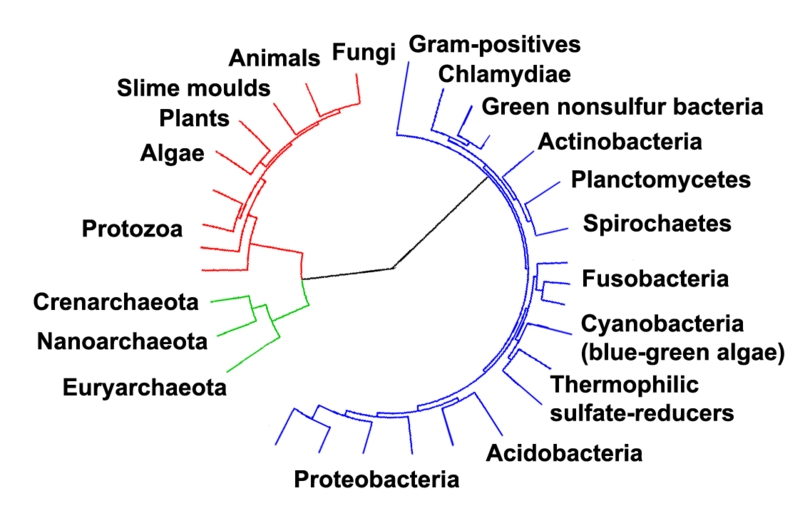
\includegraphics[angle=0,clip=true,width= \linewidth, trim = 0 0 0 0]{./pics/tree_of_life.png}}}
			\only<2>{\subfloat[Courtesy of Prof.~T.~Ueda]{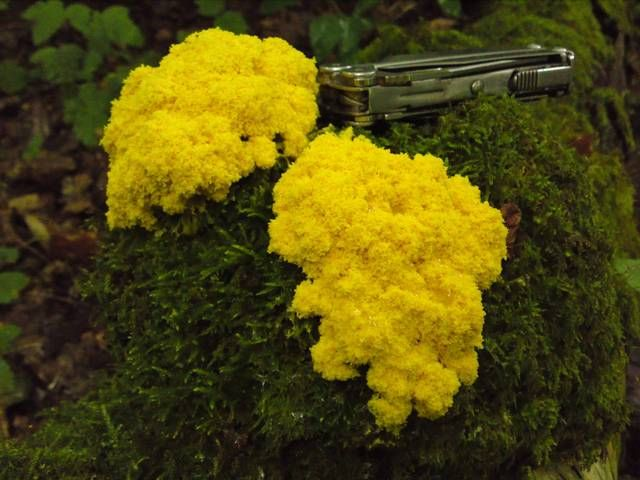
\includegraphics[angle=0,clip=true,width= \linewidth, trim = 0 0 0 0]{./pics/physarum_forest.jpg}}}
			\only<3>{\subfloat[Courtesy of Prof.~T.~Ueda]{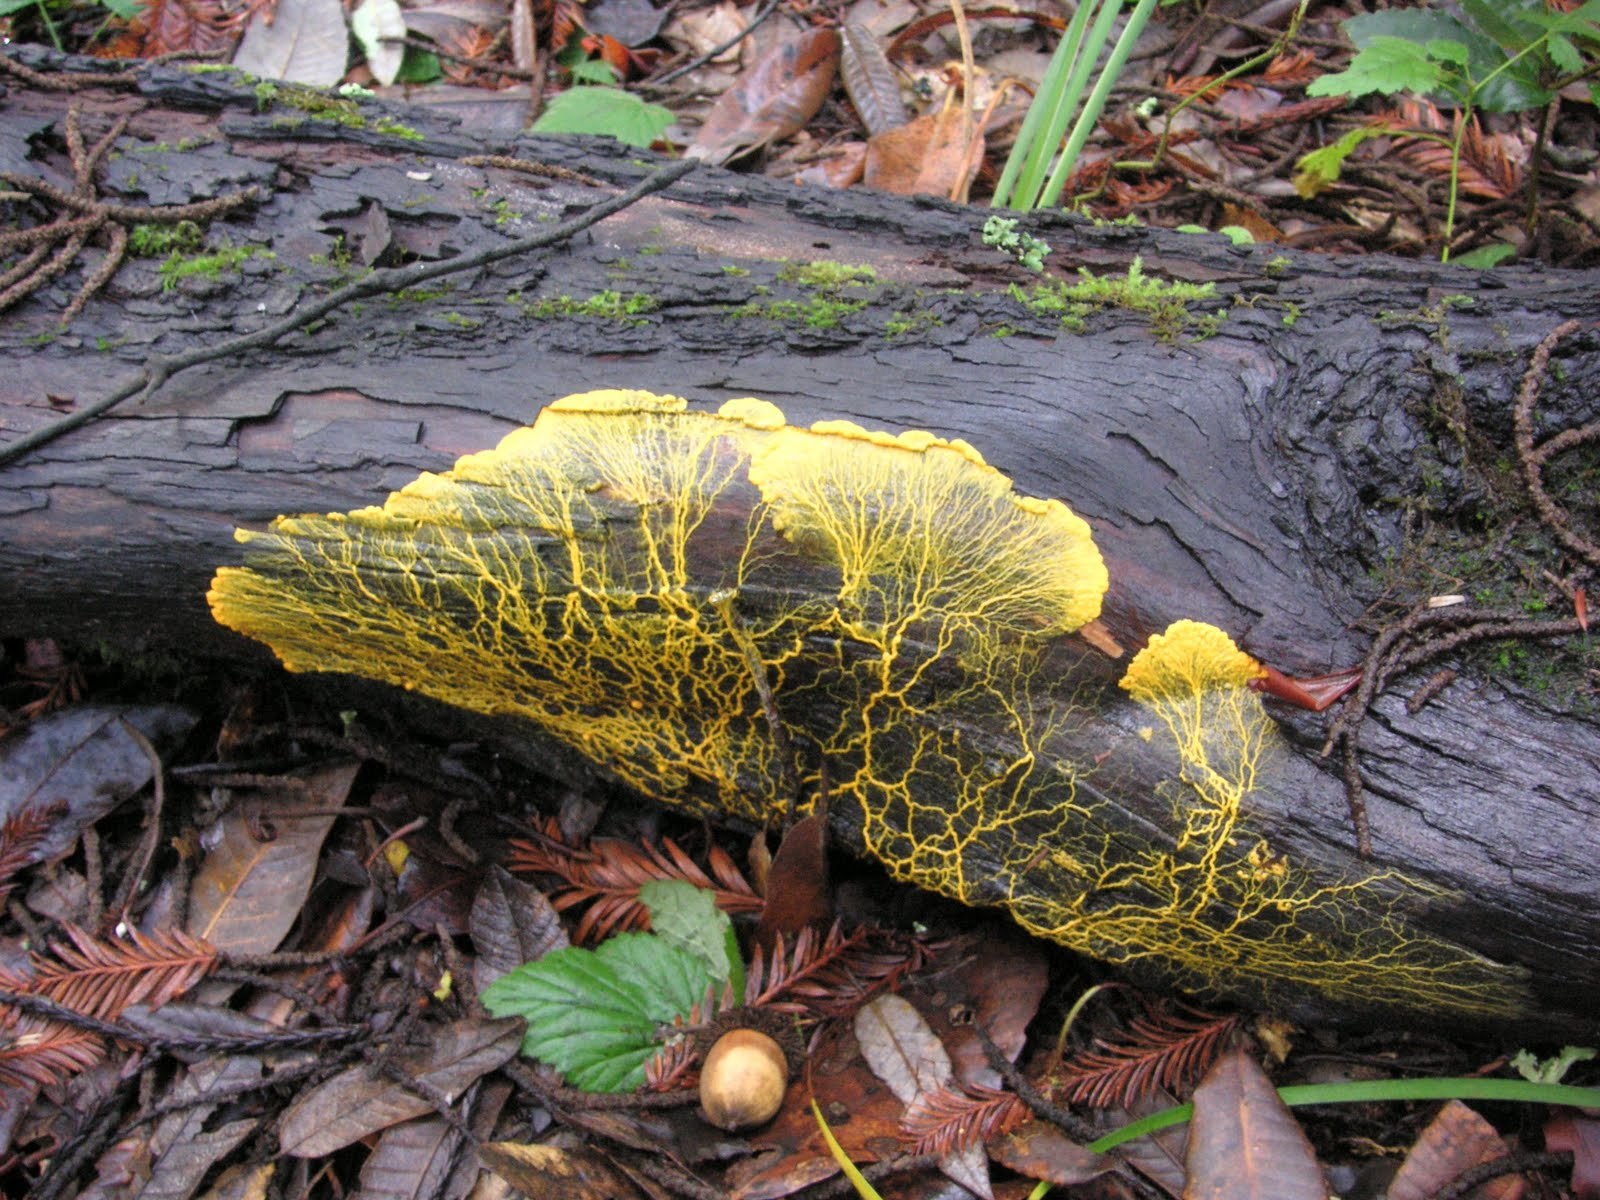
\includegraphics[angle=0,clip=true,width= \linewidth, trim = 0 0 0 0]{./pics/physarum_exploring_tree_2.jpg}}}
			\only<4>{\subfloat[Courtesy of Prof.~T.~Ueda]{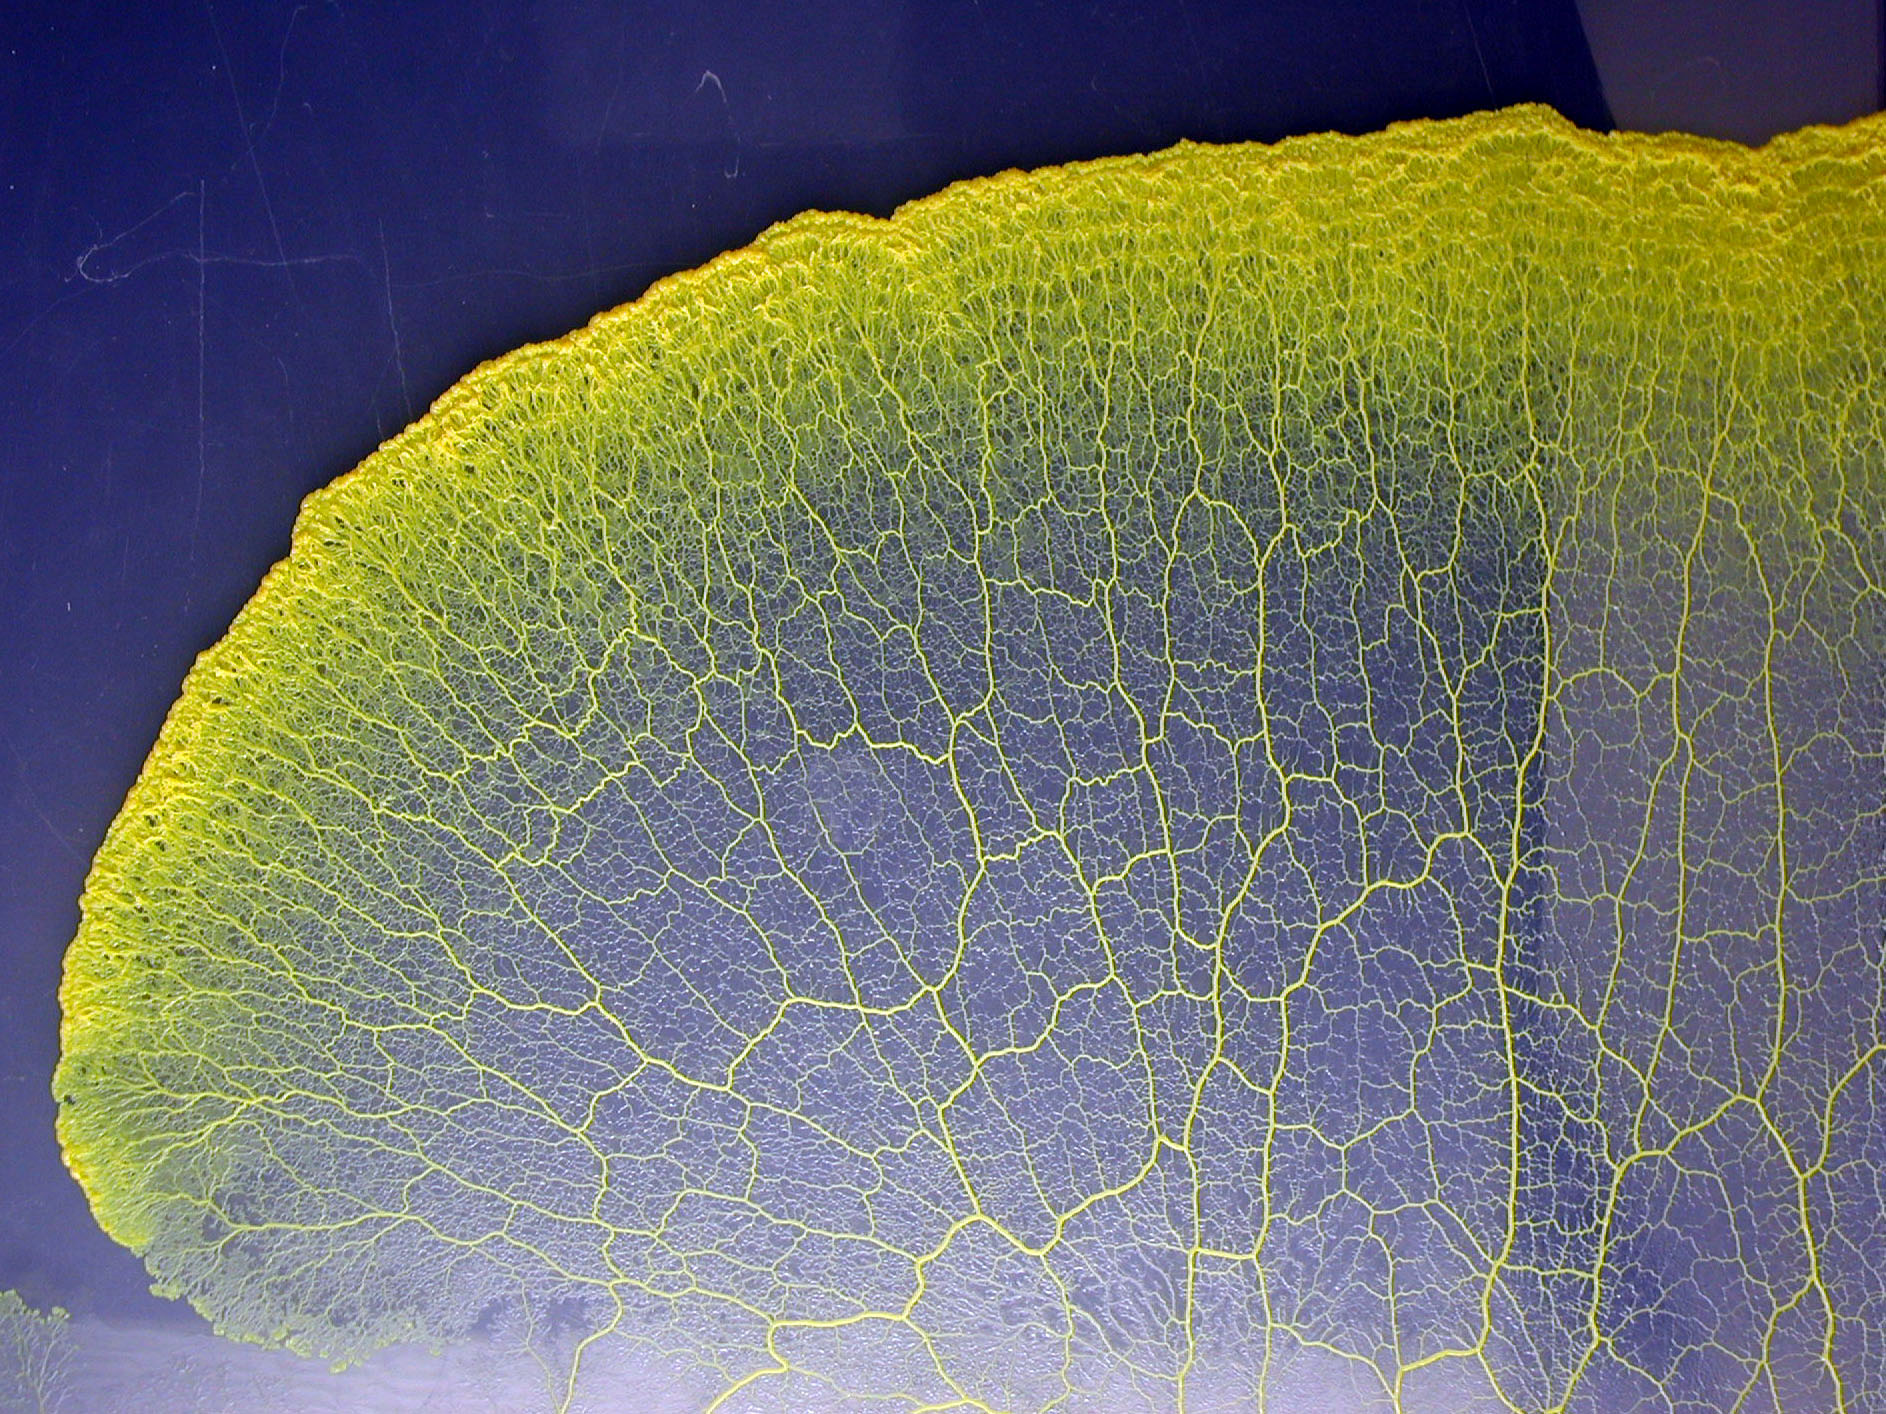
\includegraphics[angle=0,clip=true,width= \linewidth, trim = 0 0 0 0]{./pics/physarum.jpg}}}
		\end{center}
	\end{figure}
	\end{minipage} }

	\end{overprint}
	\end{column}
	\end{columns}

	\begin{alertblock}{\underline{Key Properties:}}
		Distributed dynamics, Min and Max capabilities
	\end{alertblock}
\end{frame}

\begin{frame}
    \frametitle{Natural Computing with \P} 

	\begin{columns}
	\begin{column}{4.6cm}

	\begin{overprint}

		\begin{block}{Successful approaches:}
		  \begin{itemize}
		   \item<1-> Positive feedback models/algorithms.
		   \item<2-> Many particle simulations/cellular automata. 
		   \item<3-> Steering with light.
		  \end{itemize}
		\end{block}

	\end{overprint}

	\end{column}

	\begin{column}{5cm}
	\begin{overprint}

	\testbox{
	\begin{minipage}[t]{5 cm}

	\begin{figure}[h]
		\captionsetup[subfloat]{position=bottom,labelformat=empty,font=scriptsize}
		\begin{center}
			\only<1>{\subfloat[see T. Nakagaki \etal 2006]{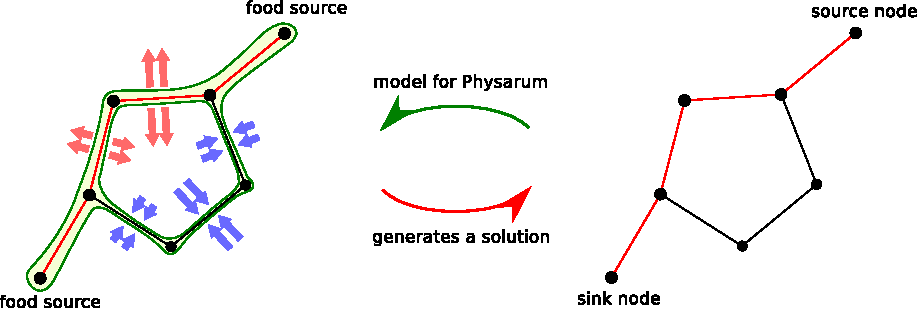
\includegraphics[angle=0,clip=true,width= 0.8\linewidth, trim = 0 0 270 0]{./pics/shortest_path_model.pdf}}}
			\only<2>{\subfloat[see J. Jones 2010]{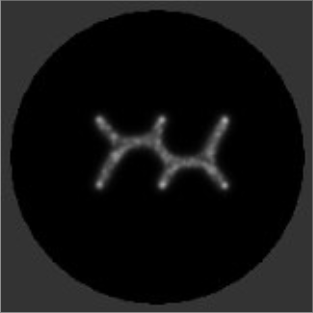
\includegraphics[angle=0,clip=true,width= 0.8\linewidth, trim = 0 0 0 0]{./pics/mst_agent.png}}}
			\only<3>{\subfloat[see M. Aono \etal 2007]{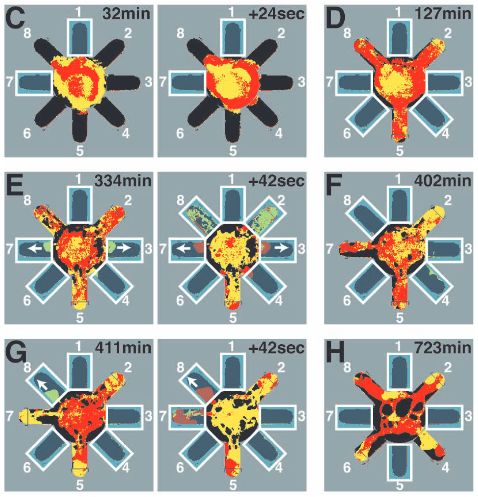
\includegraphics[angle=0,clip=true,width= 0.8\linewidth, trim = 0 0 0 0]{./pics/container_states.png}}}
		\end{center}
	\end{figure}
	\end{minipage} }


	\end{overprint}
	\end{column}
	\end{columns}
	\vspace{-0.5cm}
	\begin{alertblock}{\underline{Caveat:}}
		Existing work is focused on morphological changes in \P. Flow dynamics have largely been ignored.
	\end{alertblock}
\end{frame}

\begin{frame}
    \frametitle{What about the flows?} 

    \begin{block}{Observation:}
    	\P maintains some type of dynamic flow circulation on a changing graph in a distributed manner.
    \end{block}

     \begin{block}{Our aim:}
    	Study the networks formed by \P in order to drive the development of a distributed model of its dynamic flows.
    \end{block}

	\begin{alertblock}{\underline{Our approach:}}
		\begin{itemize}
			\item Obtain a large body of experimental data.
			\item Study network properties.
			\item Model the dynamics exhibited by \P.
		\end{itemize}
	\end{alertblock}
\end{frame}

% % 5 slides
\section{Part II: Studying the networks formed by P.~polycephalum}

\begin{frame}
    \frametitle{Experiments} 

	\begin{overprint}

		\begin{figure}[h]
		\captionsetup[subfloat]{position=bottom,labelformat=empty,font=scriptsize}
		\begin{center}
			\only<1>{\subfloat[Schematic of experimental setup.]{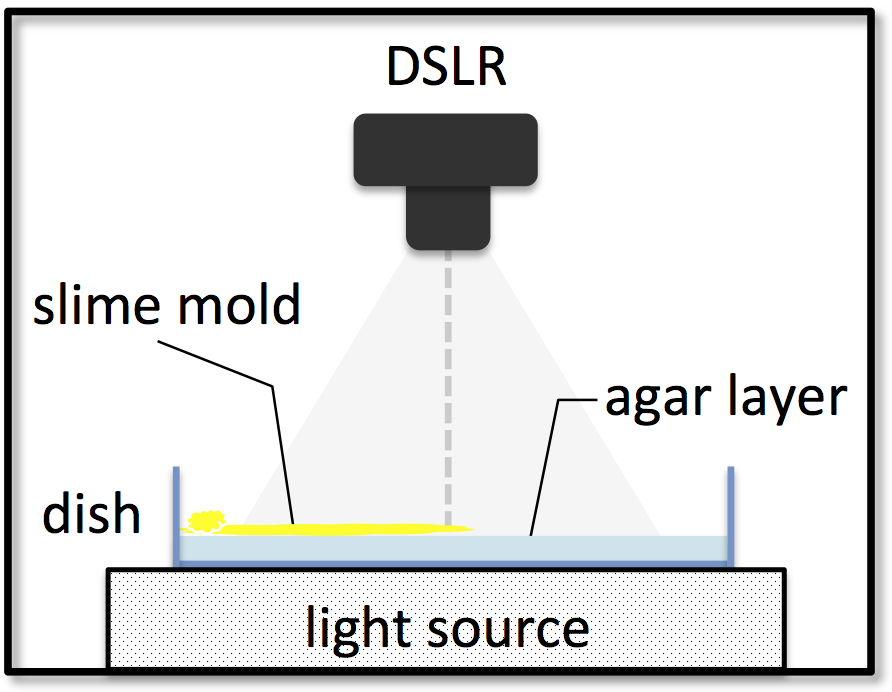
\includegraphics[angle=0,clip=true,width= 0.75\linewidth, trim = 0 0 0 0]{./pics/setup.png}}}
			\only<2>{\subfloat[Sclerotia placed in the container.]{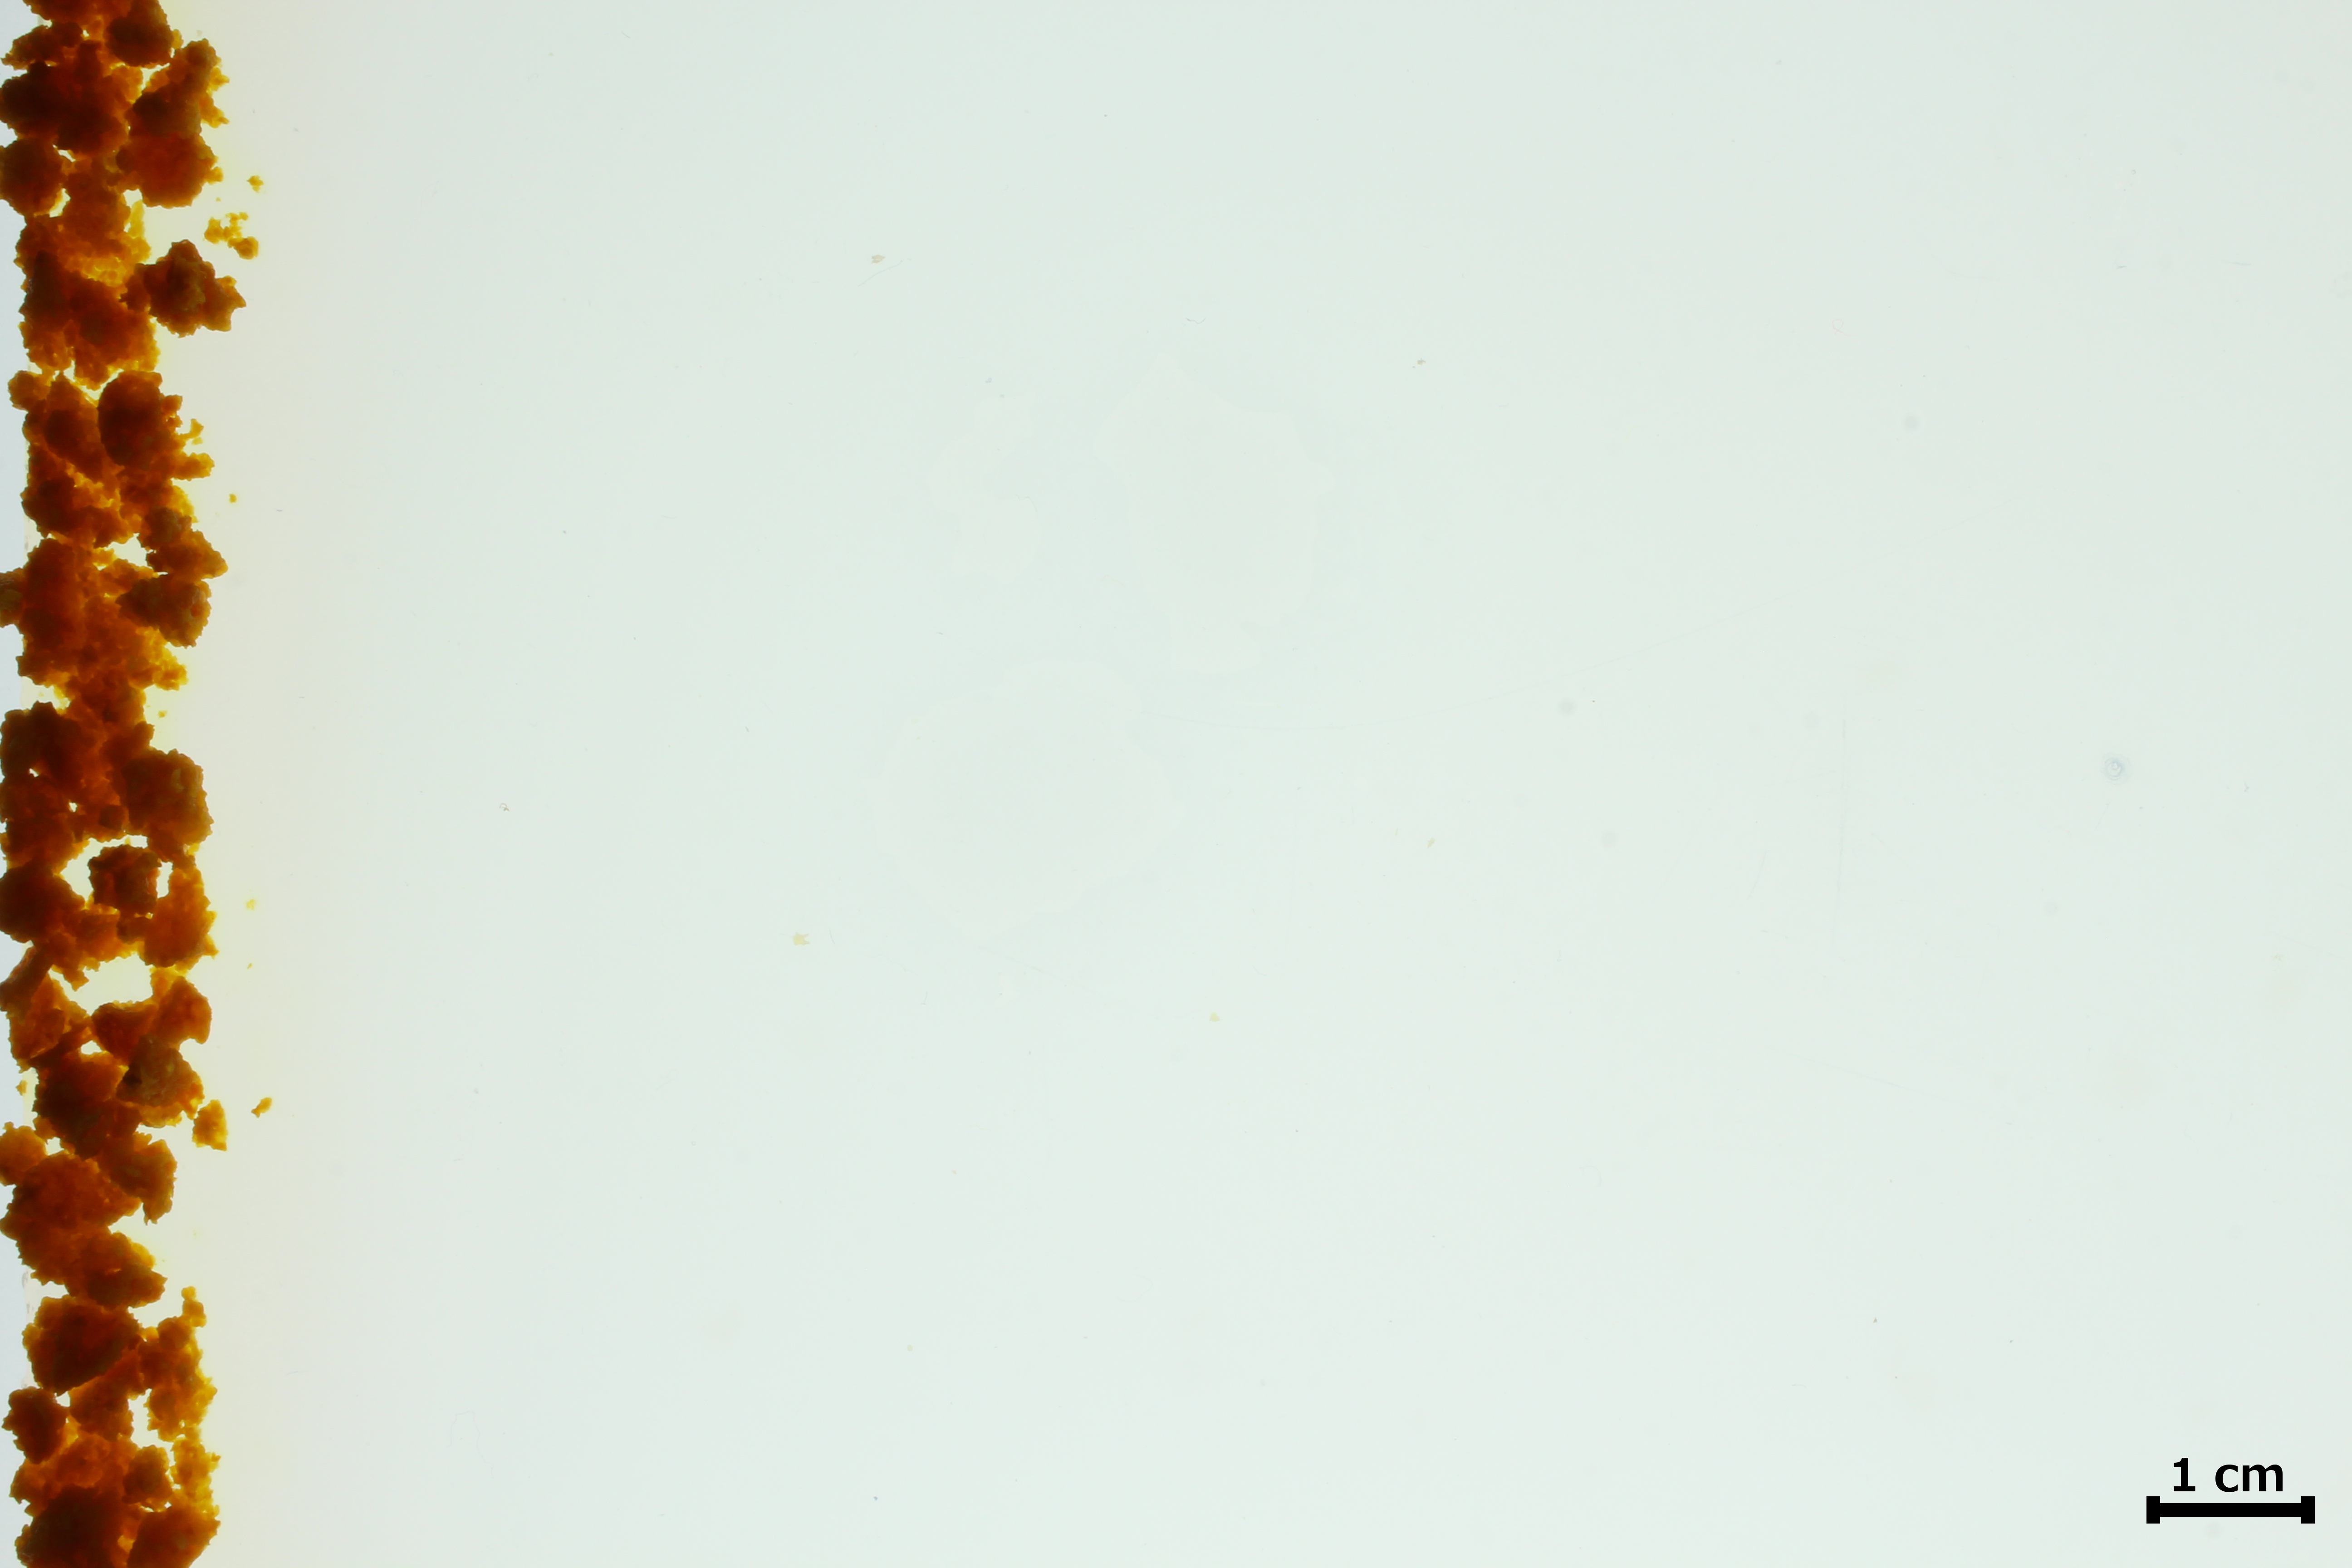
\includegraphics[angle=0,clip=true,width= \linewidth, trim = 0 0 0 0]{./pics/physarum_sequence_1.JPG}}}
			\only<3>{\subfloat[The exploring front moves on.]{\includegraphics[angle=0,clip=true,width= \linewidth, trim = 0 0 0 0]{./pics/physarum_sequence_2.JPG}}}
			\only<4>{\subfloat[A intricate network supports the front.]{\includegraphics[angle=0,clip=true,width= \linewidth, trim = 0 0 0 0]{./pics/physarum_sequence_3.JPG}}}
			\only<5>{\subfloat[A region of interest is defined.]{\includegraphics[angle=0,clip=true,width= \linewidth, trim = 0 0 0 0]{./pics/physarum_sequence_4.JPG}}}
			\only<6>{\subfloat[A graph representation of the network is computed.]{\includegraphics[angle=0,clip=true,width= \linewidth, trim = 0 0 0 0]{./pics/physarum_sequence_5.JPG}}}
		\end{center}
		\end{figure}
	\end{overprint}
\end{frame}

\begin{frame}
    \frametitle{Network Extraction From Images \tiny{\textcolor{gray}{Dirnberger~\etal,~2015}}} 

	\begin{columns}
	\begin{column}{4cm}

	\begin{overprint}

	  
		\begin{block}{}
		  \begin{itemize}
		   \item {\usebeamercolor[fg]{structure} Input:} High quality image of a network.
		   \item {\usebeamercolor[fg]{structure} Output:} Graph representation of depicted structure.
		  \end{itemize}
		\end{block}
	\end{overprint}

	\end{column}

	\begin{column}{6cm}
	\begin{overprint}


	\testbox{
	     \begin{minipage}[t]{5 cm}

	\begin{figure}[h]
	 	\captionsetup[subfloat]{position=bottom,labelformat=empty,font=scriptsize}
	    \subfloat[\NEFIs workflow.]{\includegraphics[angle=0,clip=true,width= 0.8\linewidth, trim = 0 0 0 0]{./pics/NEFI_workflow.png}}
	\end{figure}
	     \end{minipage} }

	\end{overprint}
	\end{column}
	\end{columns}

		\begin{alertblock}{\underline{Design goals:}}
		\begin{itemize}
		  	\item Combine well-known and well-implemented algorithms to obtain a new modular tool.
		  	\item Make it accessible for others (\eg non-experts).
		\end{itemize}
		\end{alertblock}
\end{frame}

\begin{frame}
    \frametitle{Analysis of \P networks} 

	\begin{block}{\data:} 
		Consists of $38$ distinct time series of \P graphs, totalling $1998$ weighted planar graphs.
	\end{block}

	\begin{block}{Goal:} 
		Obtain a catalogue of Observables that sheds light on various aspects of \P structures.
	\end{block}

	\begin{alertblock}{\underline{Scope:}}
	 \begin{itemize}
	  \item Distributions of observables and their time development.
	  \item Examples: Edge lenghts/widths, Face area/circumference and various other properties.
	 \end{itemize}
	\end{alertblock}
\end{frame}

\begin{frame}
    \frametitle{Robustness of \P networks \tiny{\textcolor{gray}{Dirnberger~\etal,~2016}}} 
   
	\begin{figure}[h]
		\captionsetup[subfloat]{position=bottom,labelformat=empty,font=scriptsize}
	     \begin{center}
	      % \testbox{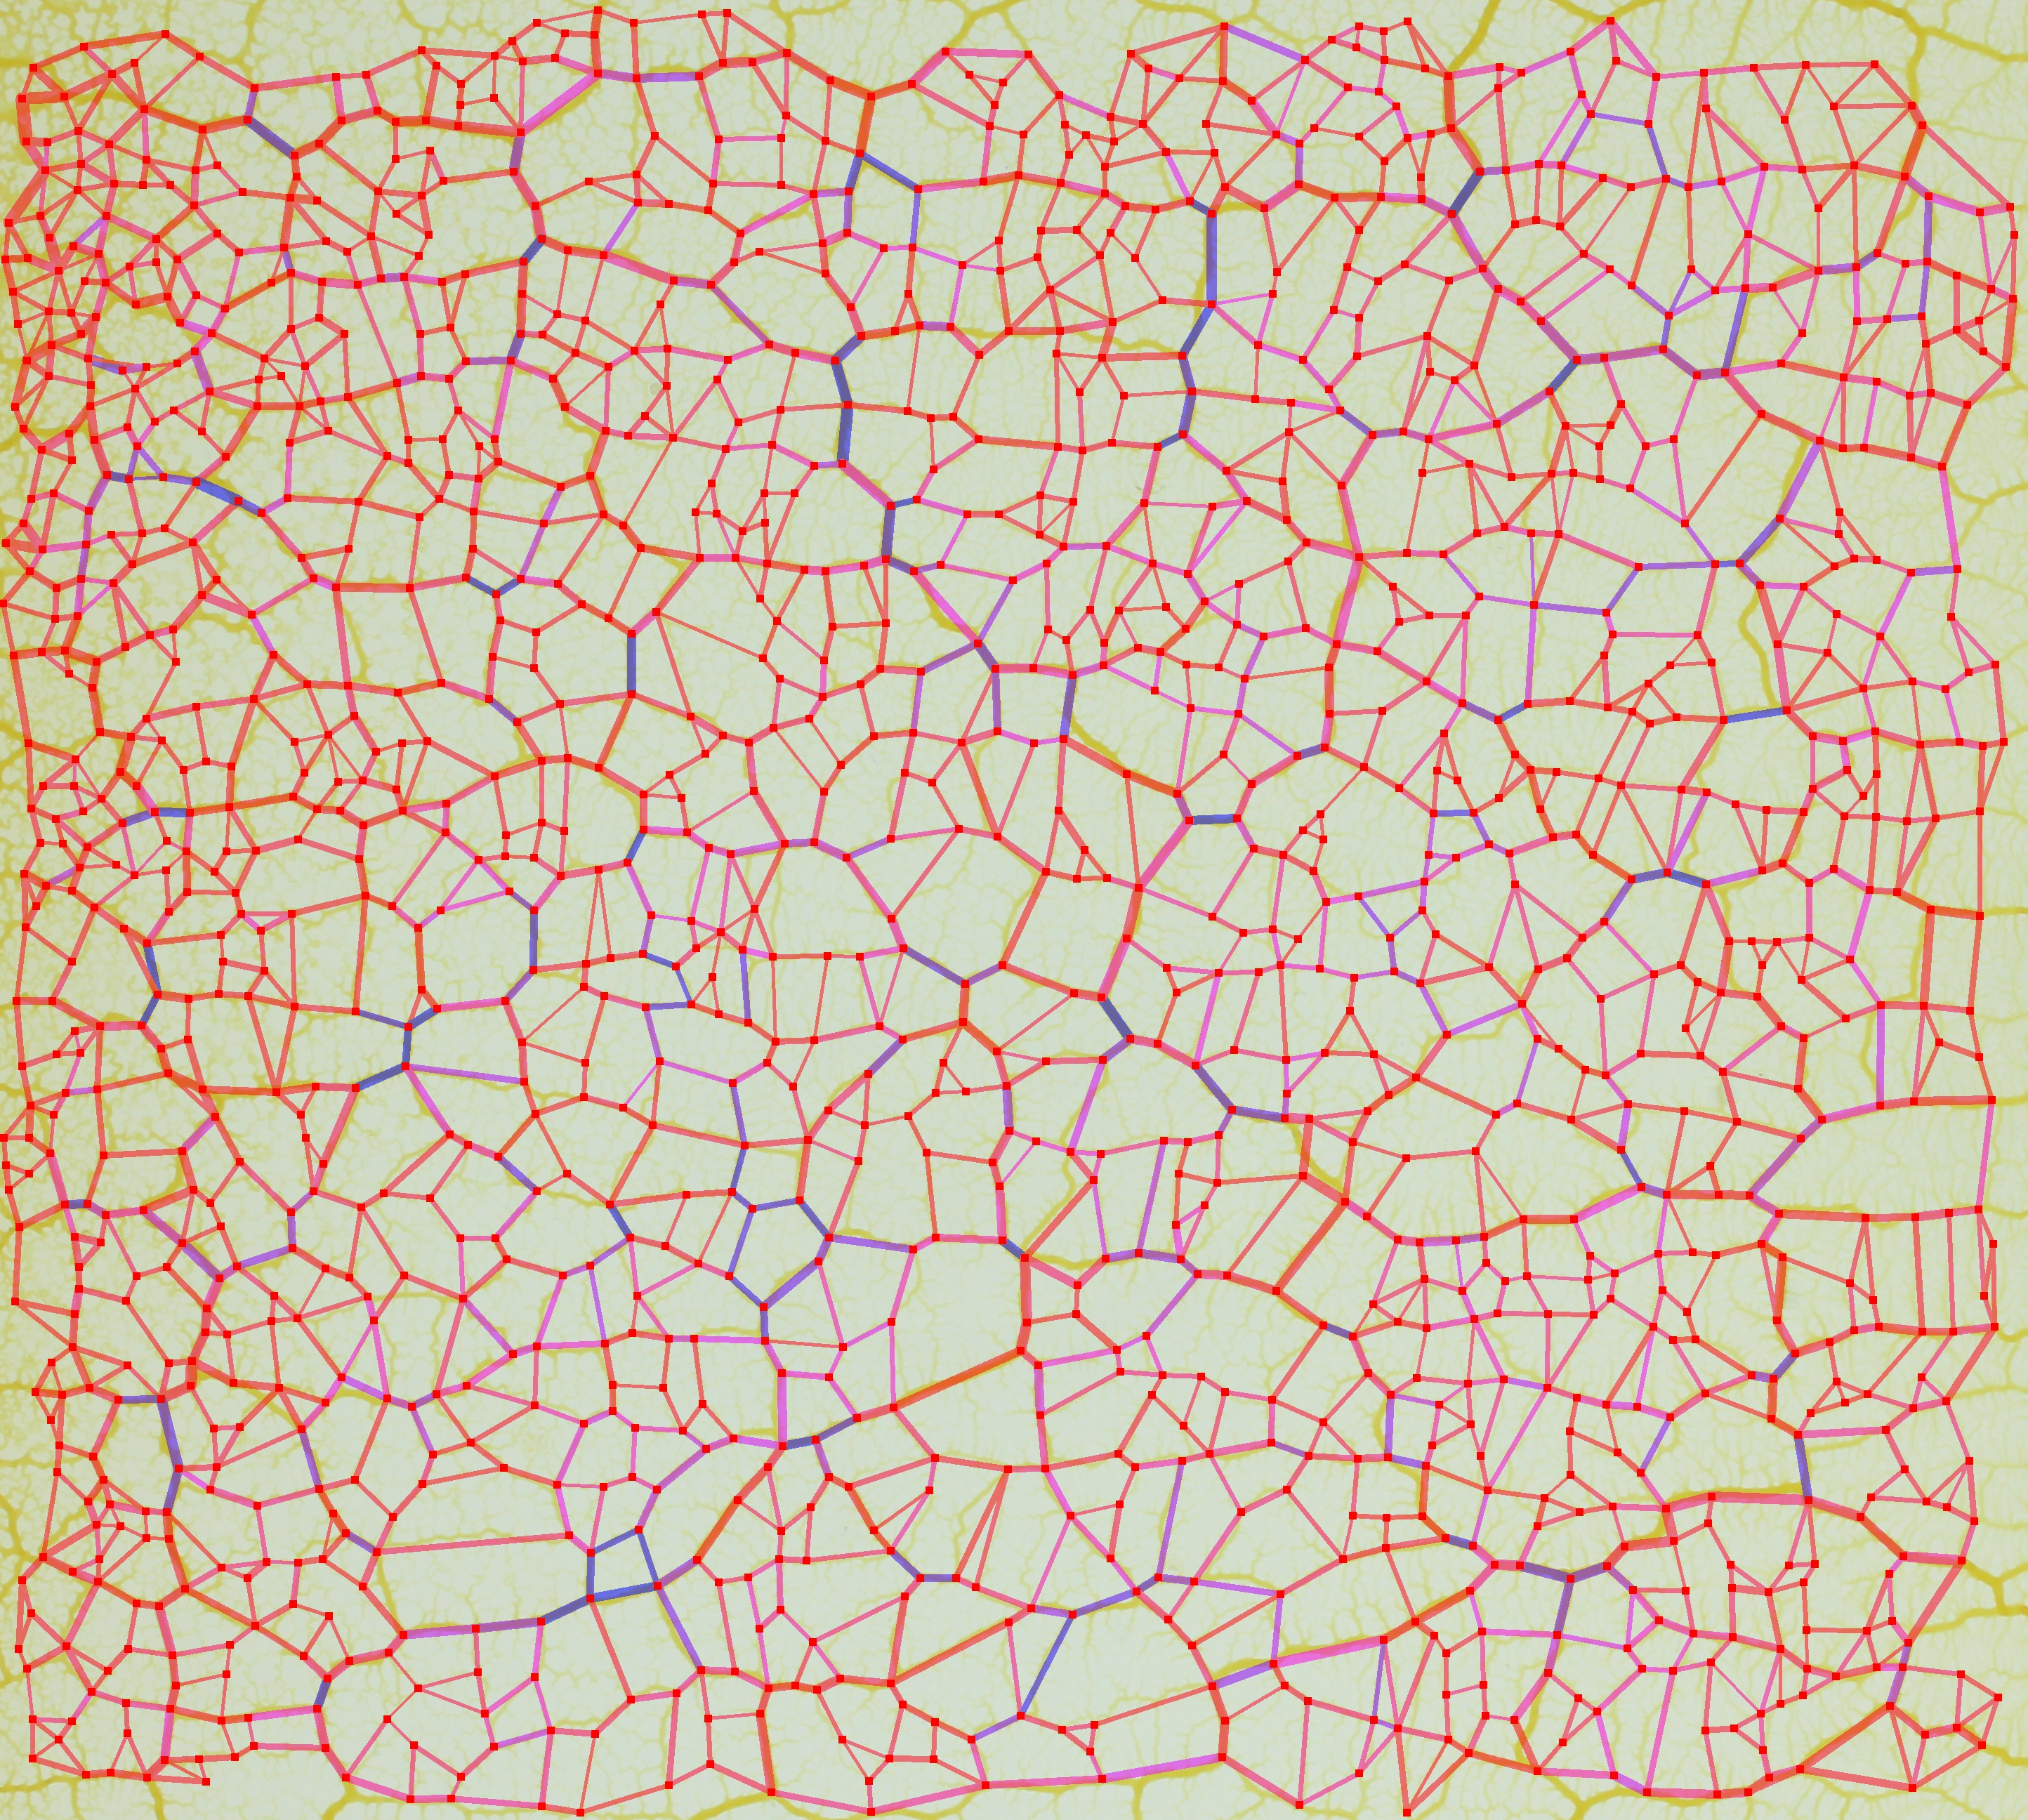
\includegraphics[angle=0,clip=true,width= 0.8\linewidth, trim = 0 0 0 0]{./pics/persistence_heat.jpg}}
	      \subfloat[Cleaned graph on-top of original image.]{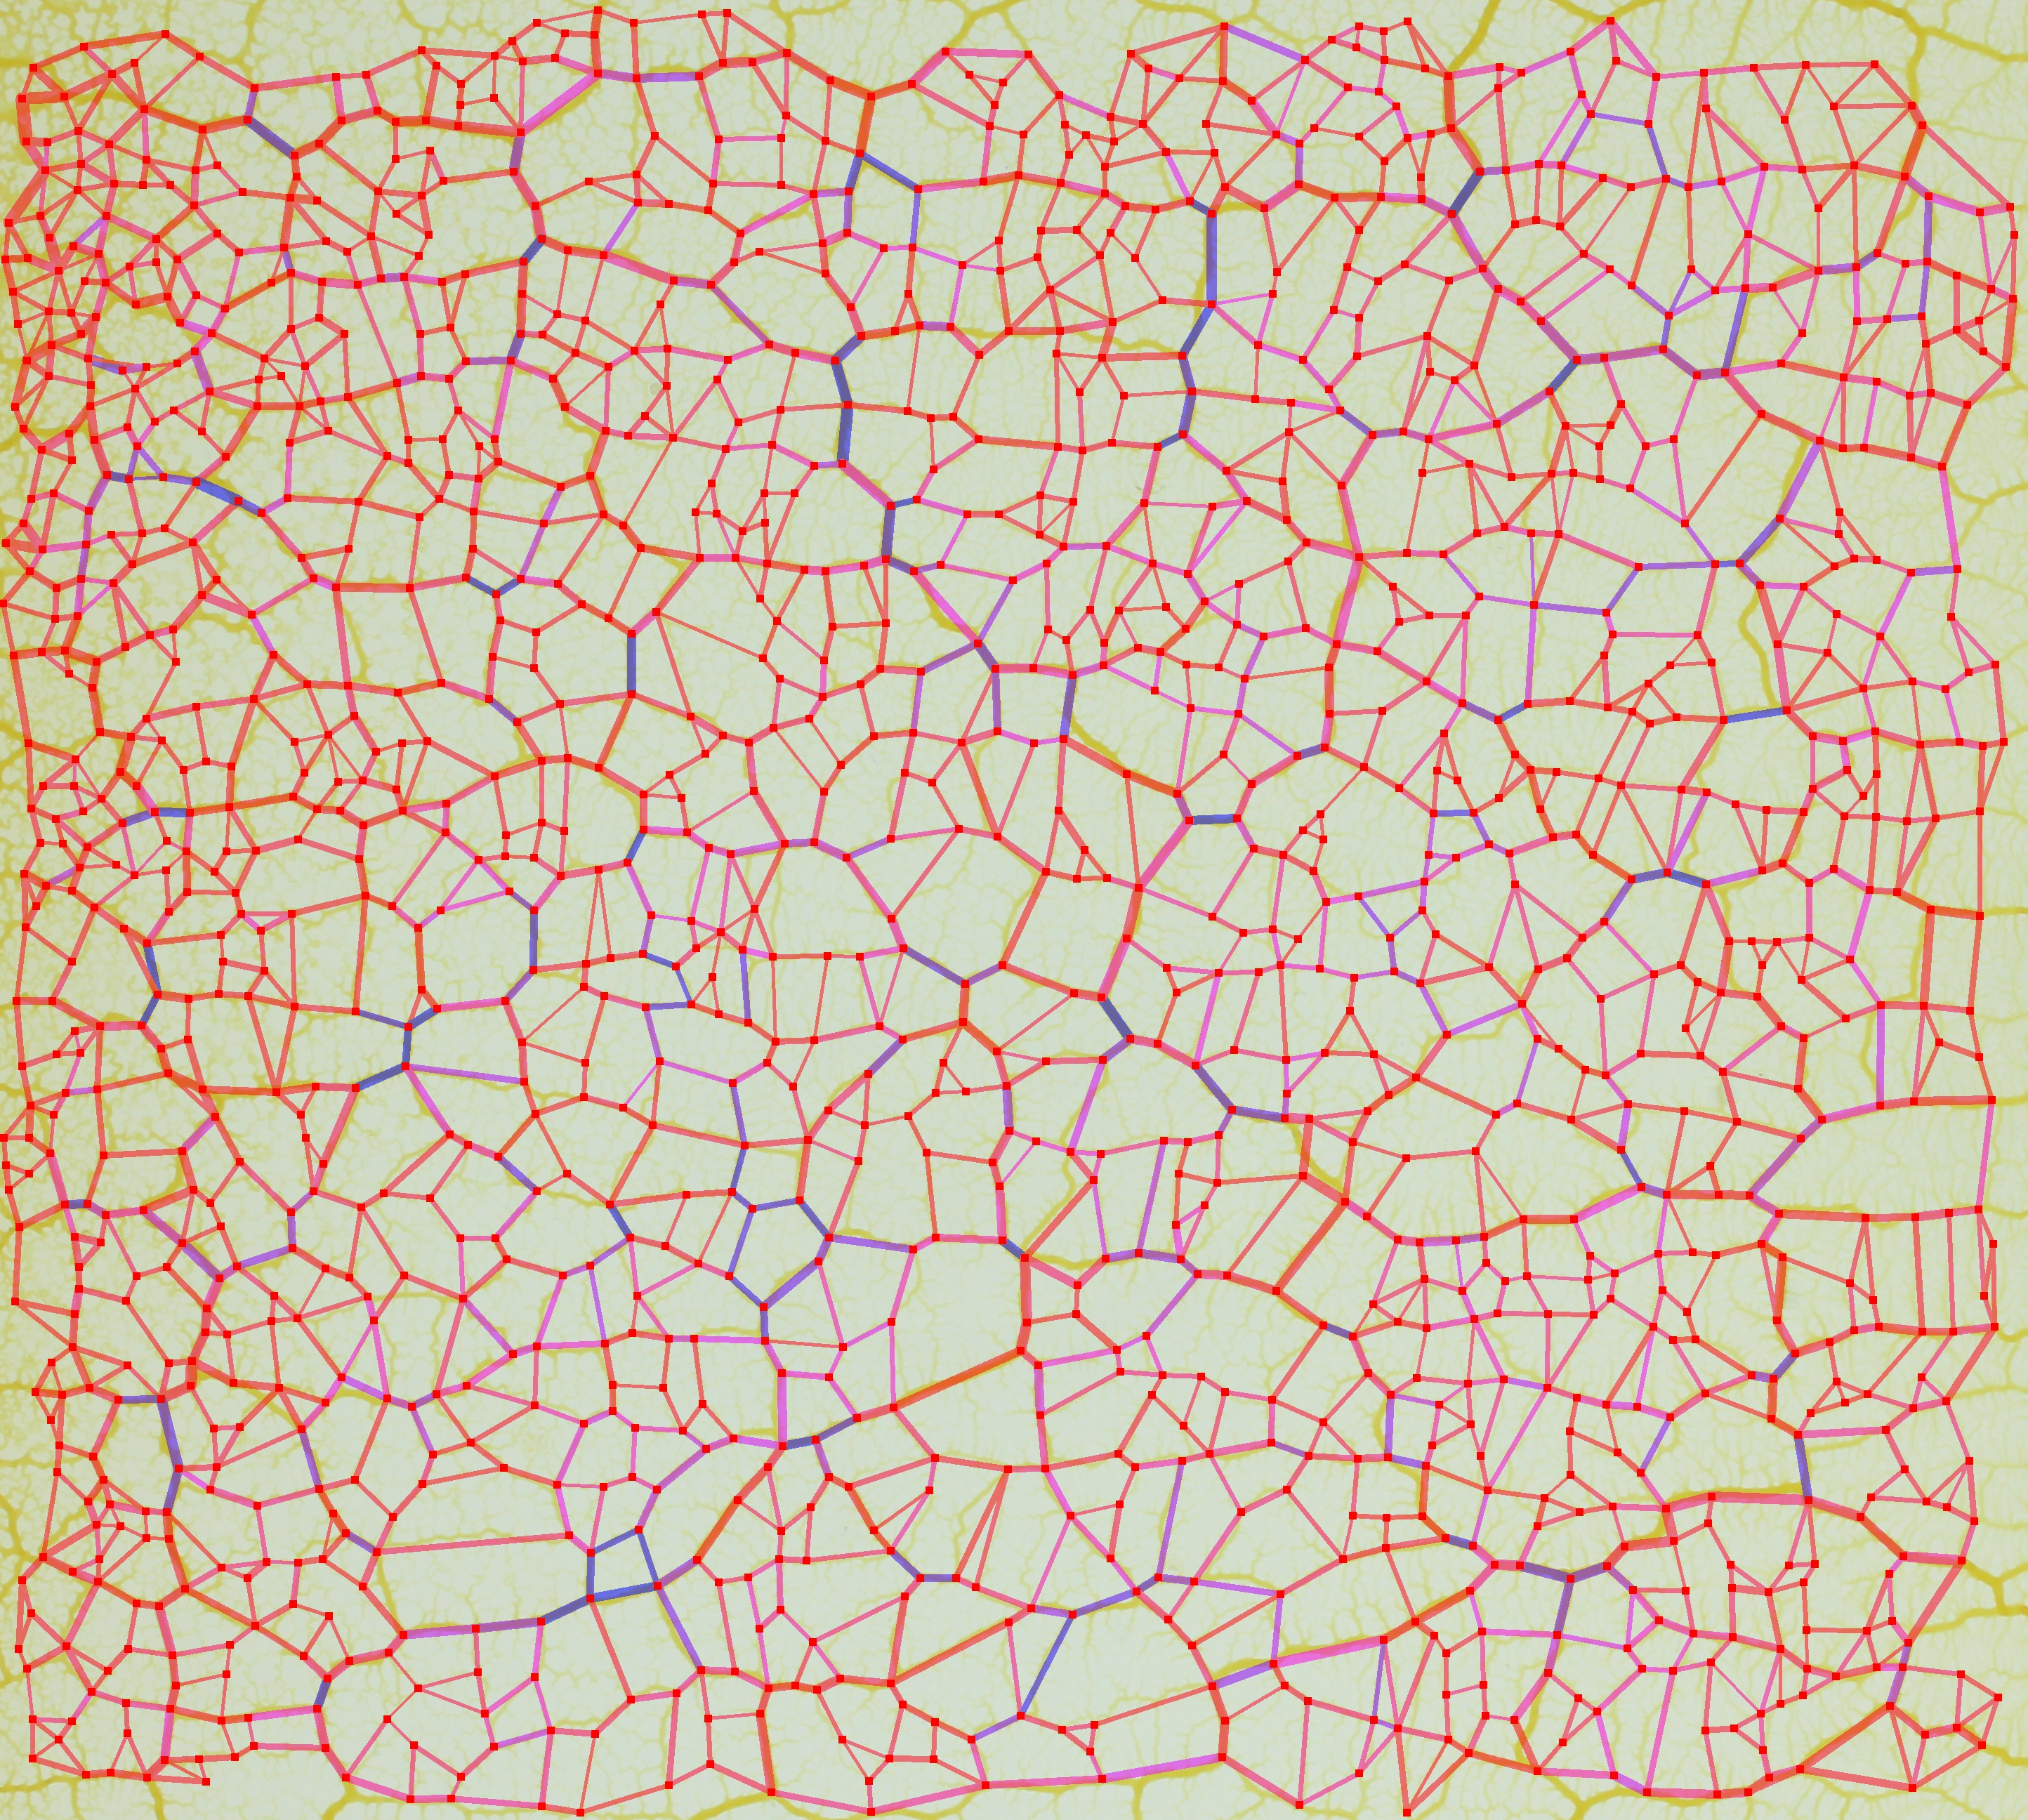
\includegraphics[angle=0,clip=true,width= 0.7\linewidth, trim = 0 0 0 0]{./pics/persistence_heat.jpg}}
	     \end{center}
	\end{figure}
\end{frame}
\begin{frame}
    \frametitle{Robustness of \P networks \tiny{\textcolor{gray}{Dirnberger~\etal,~2016}}} 
   
	\begin{figure}[h]
		 \captionsetup[subfloat]{position=bottom,labelformat=empty,font=scriptsize}
	     \begin{center}
	     \subfloat[\hspace{1cm}$p_c = 0.7118 \pm 0.0544$ for \textcolor{blue}{node percolation}
	     \hspace*{1cm}$p_c = 0.6584 \pm 0.0217$ for \textcolor{red}{edge percolation}.]{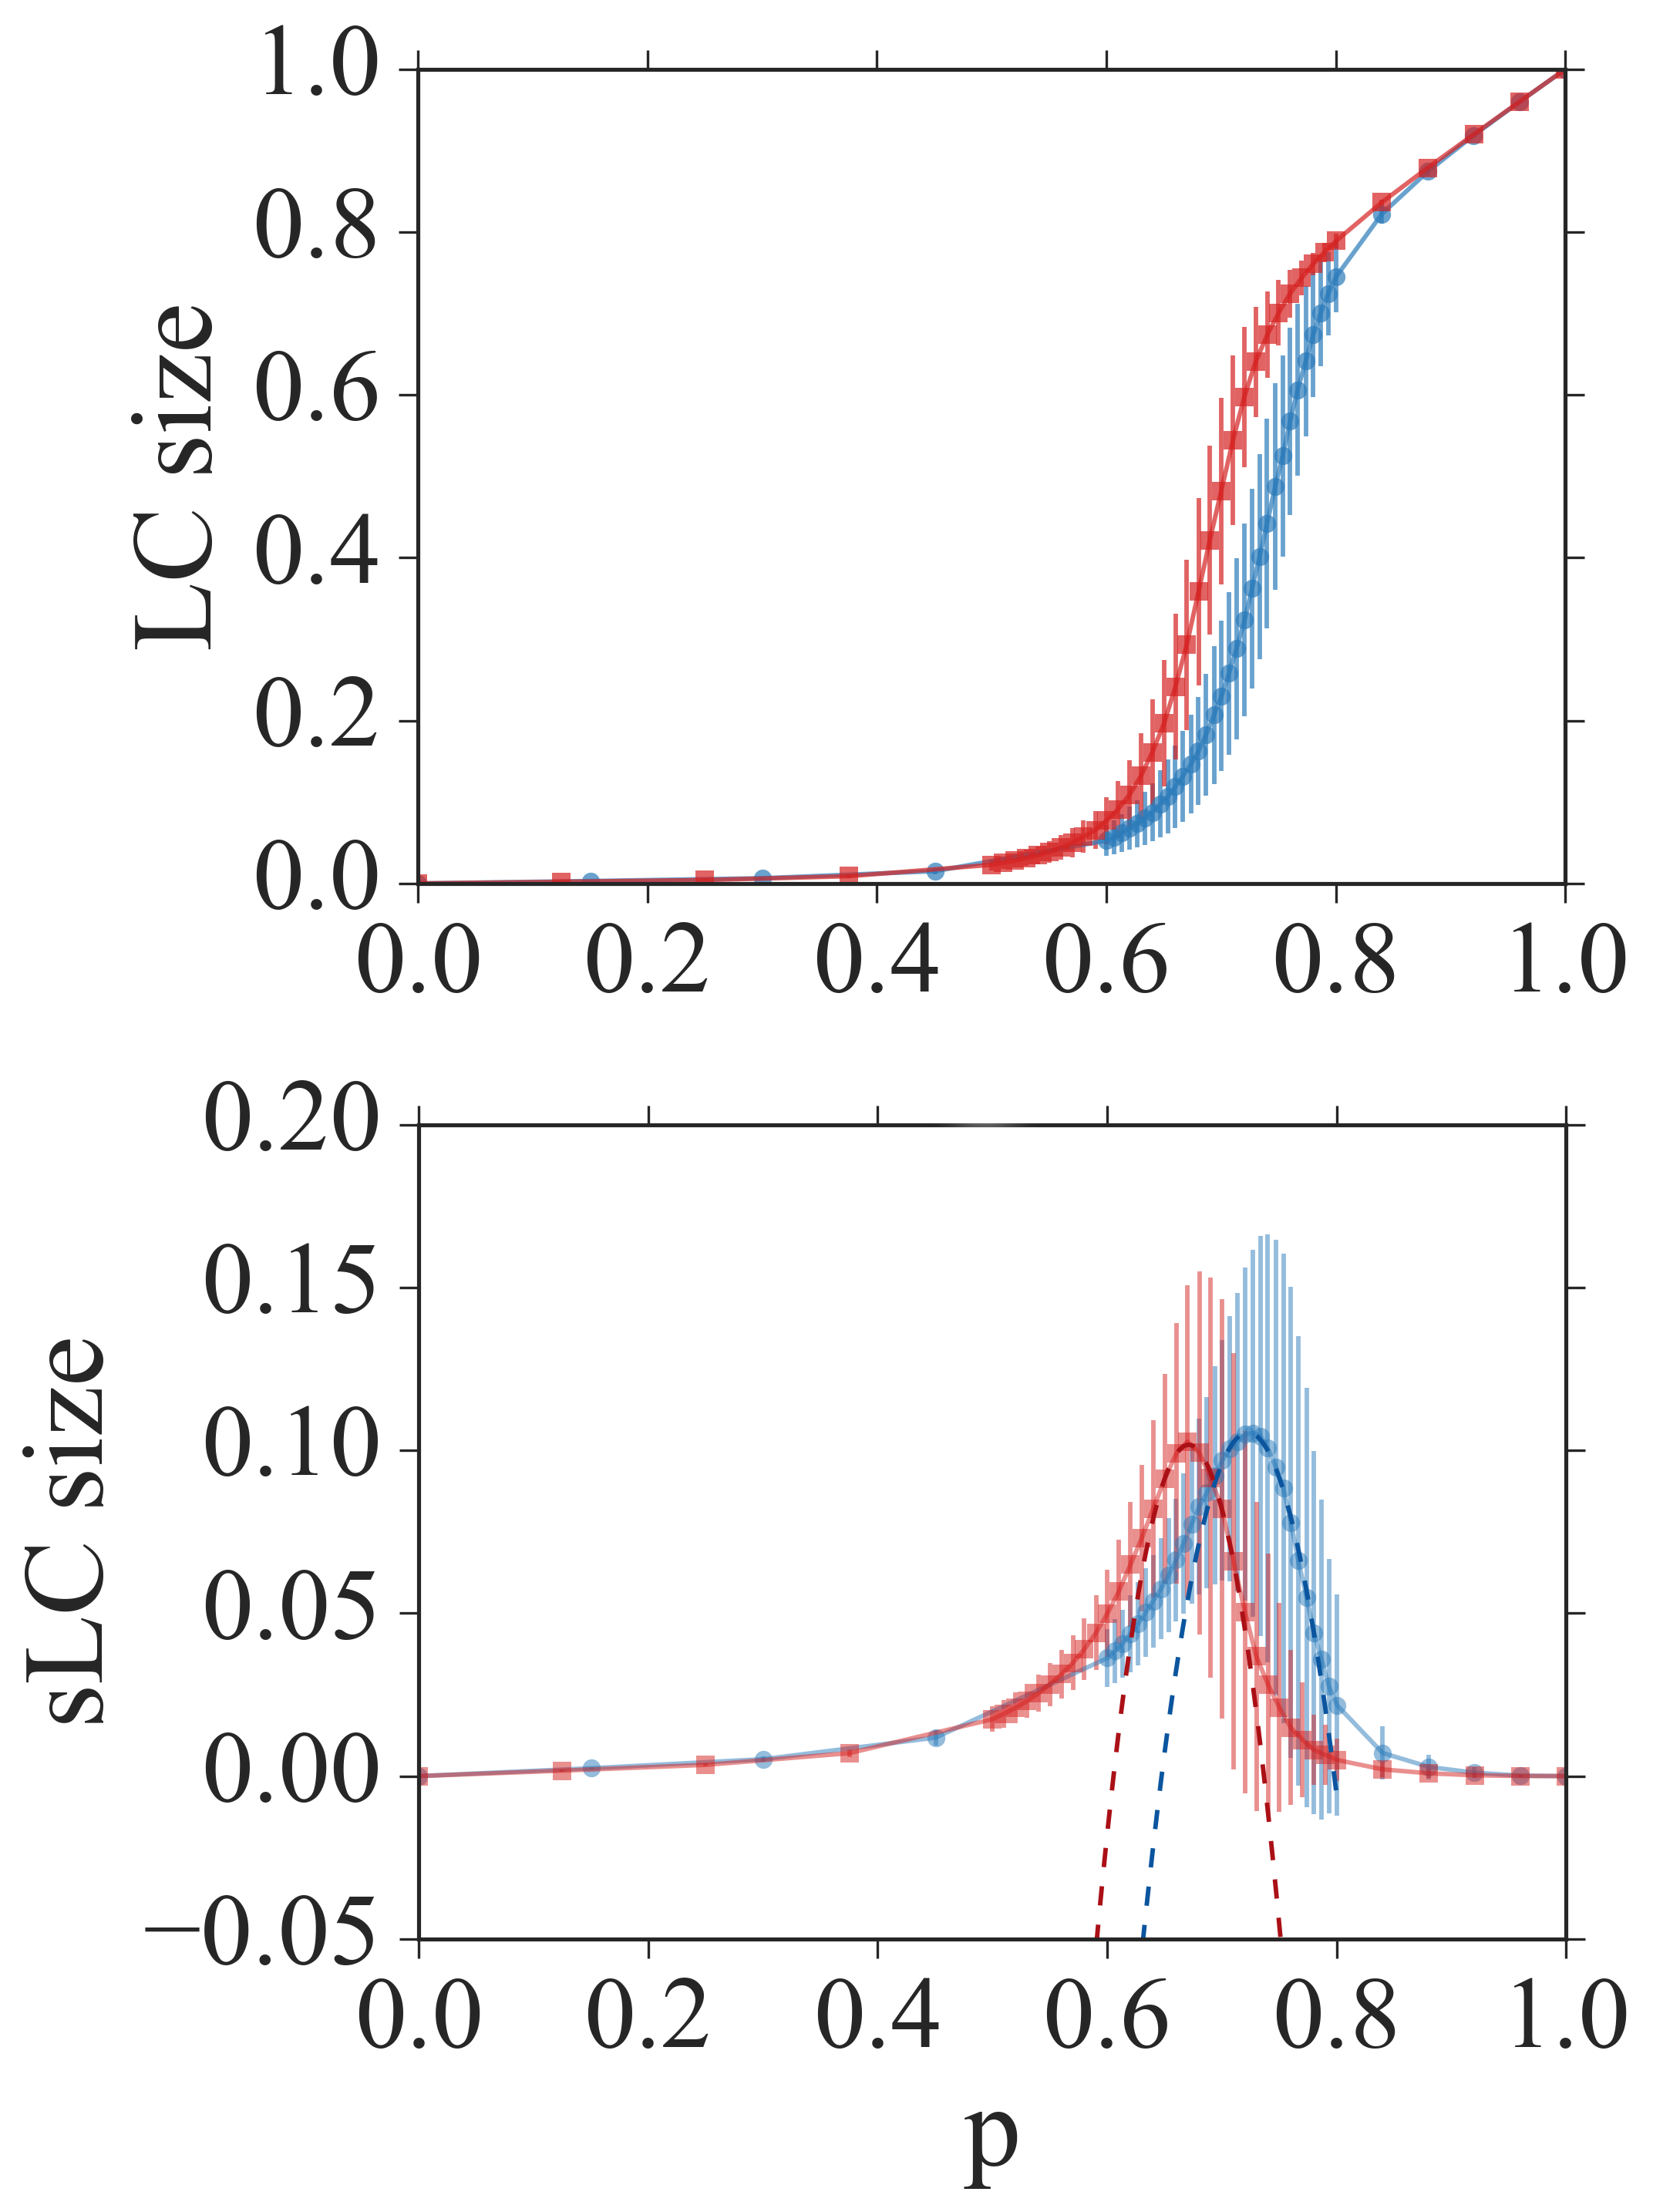
\includegraphics[angle=0,clip=true,width = 0.6\linewidth, height= 0.7\textheight, trim = 0 0 0 0]{./pics/percolation_motion22.png}}
	     \end{center}
	\end{figure}
\end{frame}

% \begin{frame}
%     \frametitle{Sharing is caring \tiny{\textcolor{gray}{Dirnberger~\etal,~2016}}} 

%     \begin{block}{\underline{Slime Mold Graph Repository:}}
%     	Collects  raw experimental data, graphs, results and useful tools.
%     \end{block}

% 	\begin{alertblock}{\underline{Motivation:}}
% 	 \begin{itemize}
% 		   \item Facilitate exchange and reuse of data.
% 		   \item Make data available to everyone.
% 		   \item Drive and evaluate modelling attempts.
% 	 \end{itemize}
% 	\end{alertblock}
% \end{frame}

% % 9 slides
\section{Part III: A distributed model of P.~polycephalum} 

\begin{frame}
    \frametitle{What we know about \P} 

	\begin{alertblock}{\underline{Desirable properties:}}
	 \begin{itemize}
	 	\item The \textbf{organism} operates in a fully distributed manner and requires no central control.
		\item The \textbf{organism} maintains a dynamic circulation of flow including flow reversals.
		\item The \textbf{organism} is robust against changes in topology.
		\item The \textbf{organism} has a degree of efficiency.
	 \end{itemize}
	\end{alertblock}
\end{frame}
\begin{frame}[noframenumbering]
    \frametitle{What we want from a model of \P} 

	\begin{alertblock}{\underline{Desirable properties:}}
	 \begin{itemize}
	 	\item The \textbf{model} operates in a fully distributed manner and requires no central control.
		\item The \textbf{model} maintains a dynamic circulation of flow including flow reversals.
		\item The \textbf{model} is robust against changes in topology.
		\item The \textbf{model} has a degree of efficiency.
	 \end{itemize}
	\end{alertblock}
\end{frame}

\begin{frame}
    \frametitle{Modelling the dynamics of \P} 

    \begin{block}{The goal:}
    	\vspace{-0.25cm}
    	Model the peristaltic pumping and obtain dynamic fluid flows similar to what is observed in \P.
    \end{block}

	\textcolor{red}{The problem:} Hydrodynamics is extremely difficult analytically!

	\begin{columns}
	\begin{column}{4.5cm}

	\begin{overprint}

		\begin{alertblock}{\underline{Solution:}}
		  \begin{itemize}
		   % \item Windkessel model.
		   \item Peristaltic pumps replaced by current controlled voltage sources.
		   \item Emergent oscillatory dynamics mimics real flow patterns.
		  \end{itemize}
		\end{alertblock}
	\end{overprint}

	\end{column}

	\begin{column}{5cm}
	\begin{overprint}

	\testbox{
	     \begin{minipage}[t]{5cm}

	\begin{figure}[h]
	 	\captionsetup[subfloat]{position=bottom,labelformat=empty,font=scriptsize}
	     \begin{center}
	      % \testbox{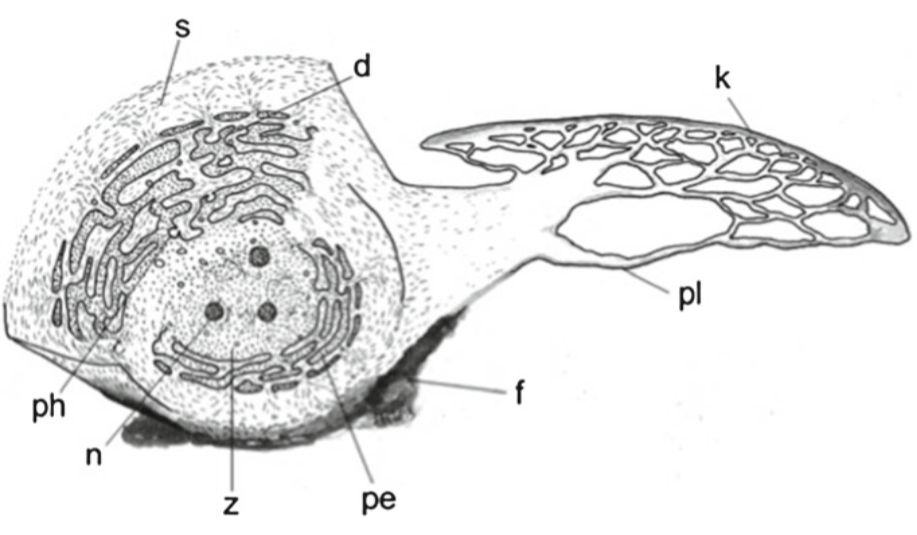
\includegraphics[angle=0,clip=true,width= 1.6\onethird, trim = 0 0 0 0]{./pics/plasmodium_hand_drawing.png}}
	      \subfloat[Courtesy of Prof.~M.~Grube.]{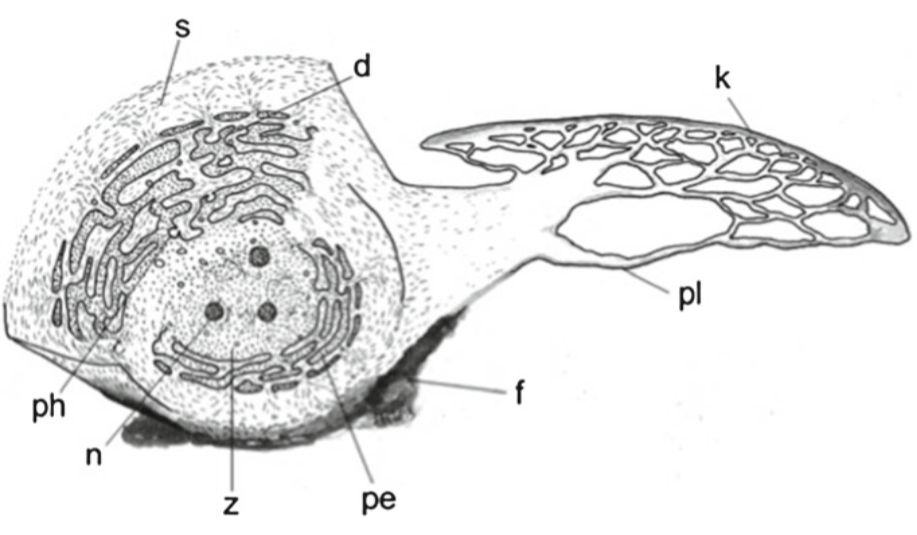
\includegraphics[angle=0,clip=true,width= \linewidth, trim = 0 0 0 0]{./pics/plasmodium_hand_drawing.png}}
	     \end{center}

	\end{figure}
	     \end{minipage} }


	\end{overprint}
	\end{column}
	\end{columns}
\end{frame}

\begin{frame}
    \frametitle{Modelling vein segments - \Pes} 
   	{\footnotesize
    \begin{table}
        \centering
        \begin{tabular}{@{} l *2l @{}}
        \toprule
         \multicolumn{1}{c}{Hydrodynamic System}    & Electrical analogue  \\ 
        \midrule
         Fluid & Charge   \\ 
         Fluid flow & Current   \\ 
         Pressure & Potential   \\ 
         Pressure difference & Voltage \\
         Viscosity & Resistance \\
         Distensibility & Capacitance \\
         Pump & Voltage souce\\
        \bottomrule
        \end{tabular}
    \end{table}
    }
	\begin{figure}
		\centering
		\begin{circuitikz}[american voltages]
		\draw
		  % rotor circuit
		  (0,0) to [short, *-] (1,0)
		  to [american controlled voltage source, cV=$u_p$] (2,0) % the pump
		  to [short, i_=$i_p$] (3,0)
		  to [R, l_=$R$] (4,0) % first R
		  to [short] (4.5,0)

		  (9,0) to [short, *-] (8,0)
		  to [american controlled voltage source, cV^=$u'_p$] (7,0) % the pump
		  to [short, i^=$i'_p$] (6,0)
		  to [R, l^=$R$] (5,0) % snd R
		  to [short] (4.5,0)
		    
		  (4.5,0) to [C, l_=$C$,i_=$i_C$,v^>=$u_{C}$] (4.5,-2)
		  to [short,-*] (0,-2)
		  
		  (4.5,-2) to [short,-*] (9,-2)

		  (0,0) to[open, v=$x$] (0,-2)

		  (9.4,0) to[open, v=$y$] (9.4,-2)

		  (4.5,-2) to (4.5,-2.0) node[ground] {};
		  
		\end{circuitikz}
		% \caption[The basic \Pe]{Electrical model of a \P vein segment. The two resistors $R$ and the capacitor $C$ form the three-element Windkessel model~\cite{olufsen2004deriving}. The two current controlled voltage sources $u_p$ and $u_p'$ augment the model to include the effects of peristaltic pumping.}
		% \label{fig:vein}
	\end{figure}
\end{frame}
\begin{frame}[noframenumbering]
	\frametitle{Modelling vein segments - \Pes} 

	\begin{figure}
		\centering
		\begin{circuitikz}[american voltages]
		\draw
		  % rotor circuit
		  (0,0) to [short, *-] (1,0)
		  to [american controlled voltage source, cV=$u_p$] (2,0) % the pump
		  to [short, i_=$i_p$] (3,0)
		  to [R, l_=$R$] (4,0) % first R
		  to [short] (4.5,0)

		  (9,0) to [short, *-] (8,0)
		  to [american controlled voltage source, cV^=$u'_p$] (7,0) % the pump
		  to [short, i^=$i'_p$] (6,0)
		  to [R, l^=$R$] (5,0) % snd R
		  to [short] (4.5,0)
		    
		  (4.5,0) to [C, l_=$C$,i_=$i_C$,v^>=$u_{C}$] (4.5,-2)
		  to [short,-*] (0,-2)
		  
		  (4.5,-2) to [short,-*] (9,-2)

		  (0,0) to[open, v=$x$] (0,-2)

		  (9.4,0) to[open, v=$y$] (9.4,-2)

		  (4.5,-2) to (4.5,-2.0) node[ground] {};
		  
		\end{circuitikz}
		% \caption[The basic \Pe]{Electrical model of a \P vein segment. The two resistors $R$ and the capacitor $C$ form the three-element Windkessel model~\cite{olufsen2004deriving}. The two current controlled voltage sources $u_p$ and $u_p'$ augment the model to include the effects of peristaltic pumping.}
		% \label{fig:vein}
	\end{figure}

    \begin{columns}
      \column{0.4\linewidth}
         \centering
         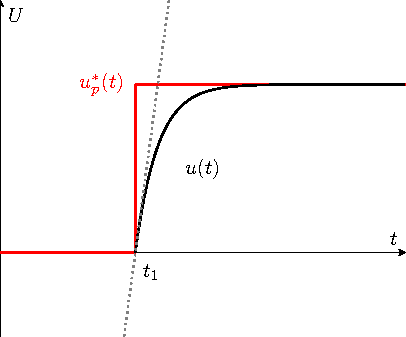
\includegraphics[width=\linewidth]{./pics/transient.pdf}
       \column{0.4\linewidth} 
          \begin{block}{Speed of response:}
          	$\dot{u}_p(t) = \alpha (u^*_p(t)-u_p(t))$
          \end{block}
     \end{columns} 
\end{frame}
\begin{frame}[noframenumbering]
	\frametitle{Modelling vein segments - \Pes} 

	\begin{figure}
		\centering
		\begin{circuitikz}[american voltages]
		\draw
		  % rotor circuit
		  (0,0) to [short, *-] (1,0)
		  to [american controlled voltage source, cV=$u_p$] (2,0) % the pump
		  to [short, i_=$i_p$] (3,0)
		  to [R, l_=$R$] (4,0) % first R
		  to [short] (4.5,0)

		  (9,0) to [short, *-] (8,0)
		  to [american controlled voltage source, cV^=$u'_p$] (7,0) % the pump
		  to [short, i^=$i'_p$] (6,0)
		  to [R, l^=$R$] (5,0) % snd R
		  to [short] (4.5,0)
		    
		  (4.5,0) to [C, l_=$C$,i_=$i_C$,v^>=$u_{C}$] (4.5,-2)
		  to [short,-*] (0,-2)
		  
		  (4.5,-2) to [short,-*] (9,-2)

		  (0,0) to[open, v=$x$] (0,-2)

		  (9.4,0) to[open, v=$y$] (9.4,-2)

		  (4.5,-2) to (4.5,-2.0) node[ground] {};
		  
		\end{circuitikz}
		% \caption[The basic \Pe]{Electrical model of a \P vein segment. The two resistors $R$ and the capacitor $C$ form the three-element Windkessel model~\cite{olufsen2004deriving}. The two current controlled voltage sources $u_p$ and $u_p'$ augment the model to include the effects of peristaltic pumping.}
		% \label{fig:vein}
	\end{figure}

    \begin{columns}
      \column{0.4\linewidth}
         \centering
         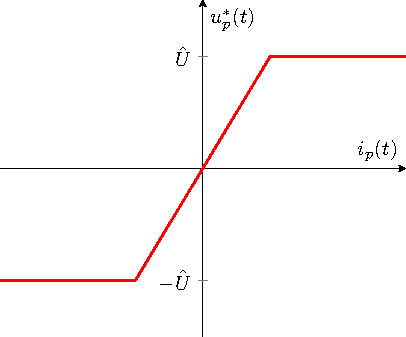
\includegraphics[width=\linewidth]{./pics/steady.pdf}
       \column{0.6\linewidth} 
          \begin{block}{Magnitude of response:}
          	$u^*_p(t) = \max(\min(\beta \cdot i_p(t),\hat{U}),-\hat{U})$
          \end{block}
     \end{columns} 
\end{frame}

\begin{frame}
    \frametitle{\Pns}

    A \Pn is a directed graph $G$ where each edge represents a \Pe. For now, all \Pes are identical.

    \begin{alertblock}{Exploration of \Pns:}

    	\begin{itemize}
    		\item Continuous version
    		\item Discretized version (Forward-Euler)
    	\end{itemize}

    \end{alertblock}

    An \emph{execution} of a \Pn is a function that maps each edge in $G$ to a signal $t \mapsto u_C(t)$.

    A \Pn $G$ \emph{converges} if all $u_{C,e}$ converge. It \emph{dies} if it converges, and for all edges $i_{p,e} = 0$ holds.
\end{frame}

\begin{frame}
	\frametitle{Example: The death of a cycle}
		\begin{figure}
			\centering
			\captionsetup[subfloat]{position=bottom,labelformat=empty,font=scriptsize}
			\subfloat[Lemma: If a cycle converges it either a) dies \dots]{\includestandalone[width=\textwidth]{./pics/standalone/cycle/cycle_dead}}%
		\end{figure}
\end{frame}
\begin{frame}[noframenumbering]
	\frametitle{Example: Counter-clockwise flow}
		\begin{figure}
			\centering
			\captionsetup[subfloat]{position=bottom,labelformat=empty,font=scriptsize}
			\subfloat[\dots \ it b) shows constant counter-clockwise flow or \dots]{\includestandalone[width=\textwidth]{./pics/standalone/cycle/cycle_cc}}%
		\end{figure}
\end{frame}
\begin{frame}[noframenumbering]
	\frametitle{Example: Clockwise flow}
		\begin{figure}
			\centering
			\captionsetup[subfloat]{position=bottom,labelformat=empty,font=scriptsize}
			\subfloat[\dots \ it c) shows constant clockwise flow.]{\includestandalone[width=\textwidth]{./pics/standalone/cycle/cycle_cw}}%
		\end{figure}
\end{frame}

\begin{frame}
	\frametitle{Example: Synchronisation on a tree}
		\begin{figure}
			\centering
			\captionsetup[subfloat]{position=bottom,labelformat=empty,font=scriptsize}
			\subfloat[Lemma: If a tree converges it dies.]{\includestandalone[width=\textwidth]{./pics/standalone/tree/tree}}%
		\end{figure}
\end{frame}

% \begin{frame}
% 	\frametitle{Example: Two coupled cycles}
% 		\begin{figure}
% 			\centering
% 			\captionsetup[subfloat]{position=bottom,labelformat=empty,font=scriptsize}
% 			\subfloat[Model behaviour mimics experimental observations of A. Takamatsu \etal, 2000.]{\includestandalone[width=\textwidth]{./pics/standalone/coupled/1}}%
% 		\end{figure}
% \end{frame}
% \begin{frame}[noframenumbering]
% 	\frametitle{Example: Two coupled cycles}
% 		\begin{figure}
% 			\centering
% 			\captionsetup[subfloat]{position=bottom,labelformat=empty,font=scriptsize}
% 			\subfloat[Model behaviour mimics experimental observations of A. Takamatsu \etal, 2000.]{\includestandalone[width=\textwidth]{./pics/standalone/coupled/2}}%
% 		\end{figure}
% \end{frame}
\begin{frame}
	\frametitle{Example: Two coupled cycles}
		\begin{figure}
			\centering
			\captionsetup[subfloat]{position=bottom,labelformat=empty,font=scriptsize}
			\subfloat[Model behaviour mimics experimental observations of A. Takamatsu \etal, 2000.]{\includestandalone[width=\textwidth]{./pics/standalone/coupled/3}}%
		\end{figure}
\end{frame}

\begin{frame}
	\frametitle{A model at the cross-roads}

	\begin{block}{Status Quo:}
		We have obtained a novel distributed model that mimics the flow dynamics of \P!
	\end{block}
	\begin{alertblock}{\underline{How to proceed?}}
		\begin{itemize}
			\item Try to use the flow reversals exhibited in the model to solve a problem (M. Függer, M. Grube).
			\item Try to improve the realism of the model to obtain a more physical description.
		\end{itemize}
	\end{alertblock}

	Both approaches are worthwhile, require specialist input and continued interdisciplinary effort.
\end{frame}

\begin{frame}
	\frametitle{Summary}

	\begin{itemize}
		\item Illustrated how the distributed nature of \Pp renders it a promising candidate for Natural Computing.
		\item Presented our efforts to better understand the networks formed by the organism.
		% \item Emphasized how our work supports the community.
		\item Sketched our modelling attempts and demonstrated the validity of the approach.
		\item Briefly discussed possible avenues for future developments.
	\end{itemize}
\end{frame}
\begin{frame}[noframenumbering]
	\frametitle{} 

	\begin{columns}
	\begin{column}{5cm}

	\begin{overprint}
		\begin{center}
			{\usebeamercolor[fg]{structure} Thank you.}
		\end{center}
	\end{overprint}

	\end{column}

	\begin{column}{5cm}
	\begin{overprint}


	     \begin{minipage}[t]{5 cm}

			\begin{figure}[h]
			 
			     \begin{center}
			      	\testbox{\includegraphics[angle=0,clip=true,width= 1.25\onethird, trim = 0 0 270 0]{./pics/physarum_art.JPG}}
			     \end{center}

			\end{figure}
	     \end{minipage}

	\end{overprint}
	\end{column}
	\end{columns}
\end{frame}

% back up slides go here

\begin{frame}[noframenumbering]
\end{frame}

\begin{frame}
	\frametitle{\NEFIs pipeline}

	\begin{figure}
		\centering
		\captionsetup[subfloat]{position=bottom,labelformat=empty,font=scriptsize}
		\subfloat[][]{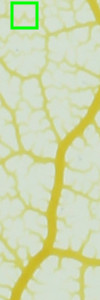
\includegraphics[width=0.13\linewidth,keepaspectratio]{./pics/pipeline/input.jpg}\label{fig:pipeline:input}}\qquad
		\subfloat[][]{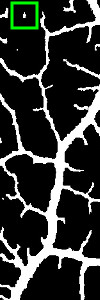
\includegraphics[width=0.13\linewidth,keepaspectratio]{./pics/pipeline/segmented.jpg}\label{fig:pipeline:segmented}}\qquad
		\subfloat[][]{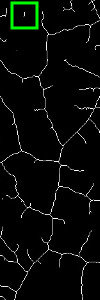
\includegraphics[width=0.13\linewidth,keepaspectratio]{./pics/pipeline/skeleton.jpg}\label{fig:pipeline:skeleton}}\qquad
		\subfloat[][]{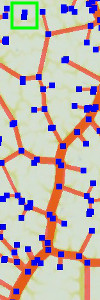
\includegraphics[width=0.13\linewidth,keepaspectratio]{./pics/pipeline/full_graph.jpg}\label{fig:pipeline:full_graph}}\qquad
		\subfloat[][]{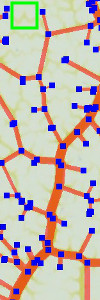
\includegraphics[width=0.13\linewidth,keepaspectratio]{./pics/pipeline/largest_component.jpg}\label{fig:pipeline:largest_component}}\qquad
		\caption[]{\NEFIs pipeline steps.}
	\end{figure}
\end{frame}

\begin{frame}
	\frametitle{\NEFIs pipeline}

	\begin{figure}
		\centering
		\captionsetup[subfloat]{position=bottom,labelformat=empty,font=scriptsize}
		\subfloat[][]{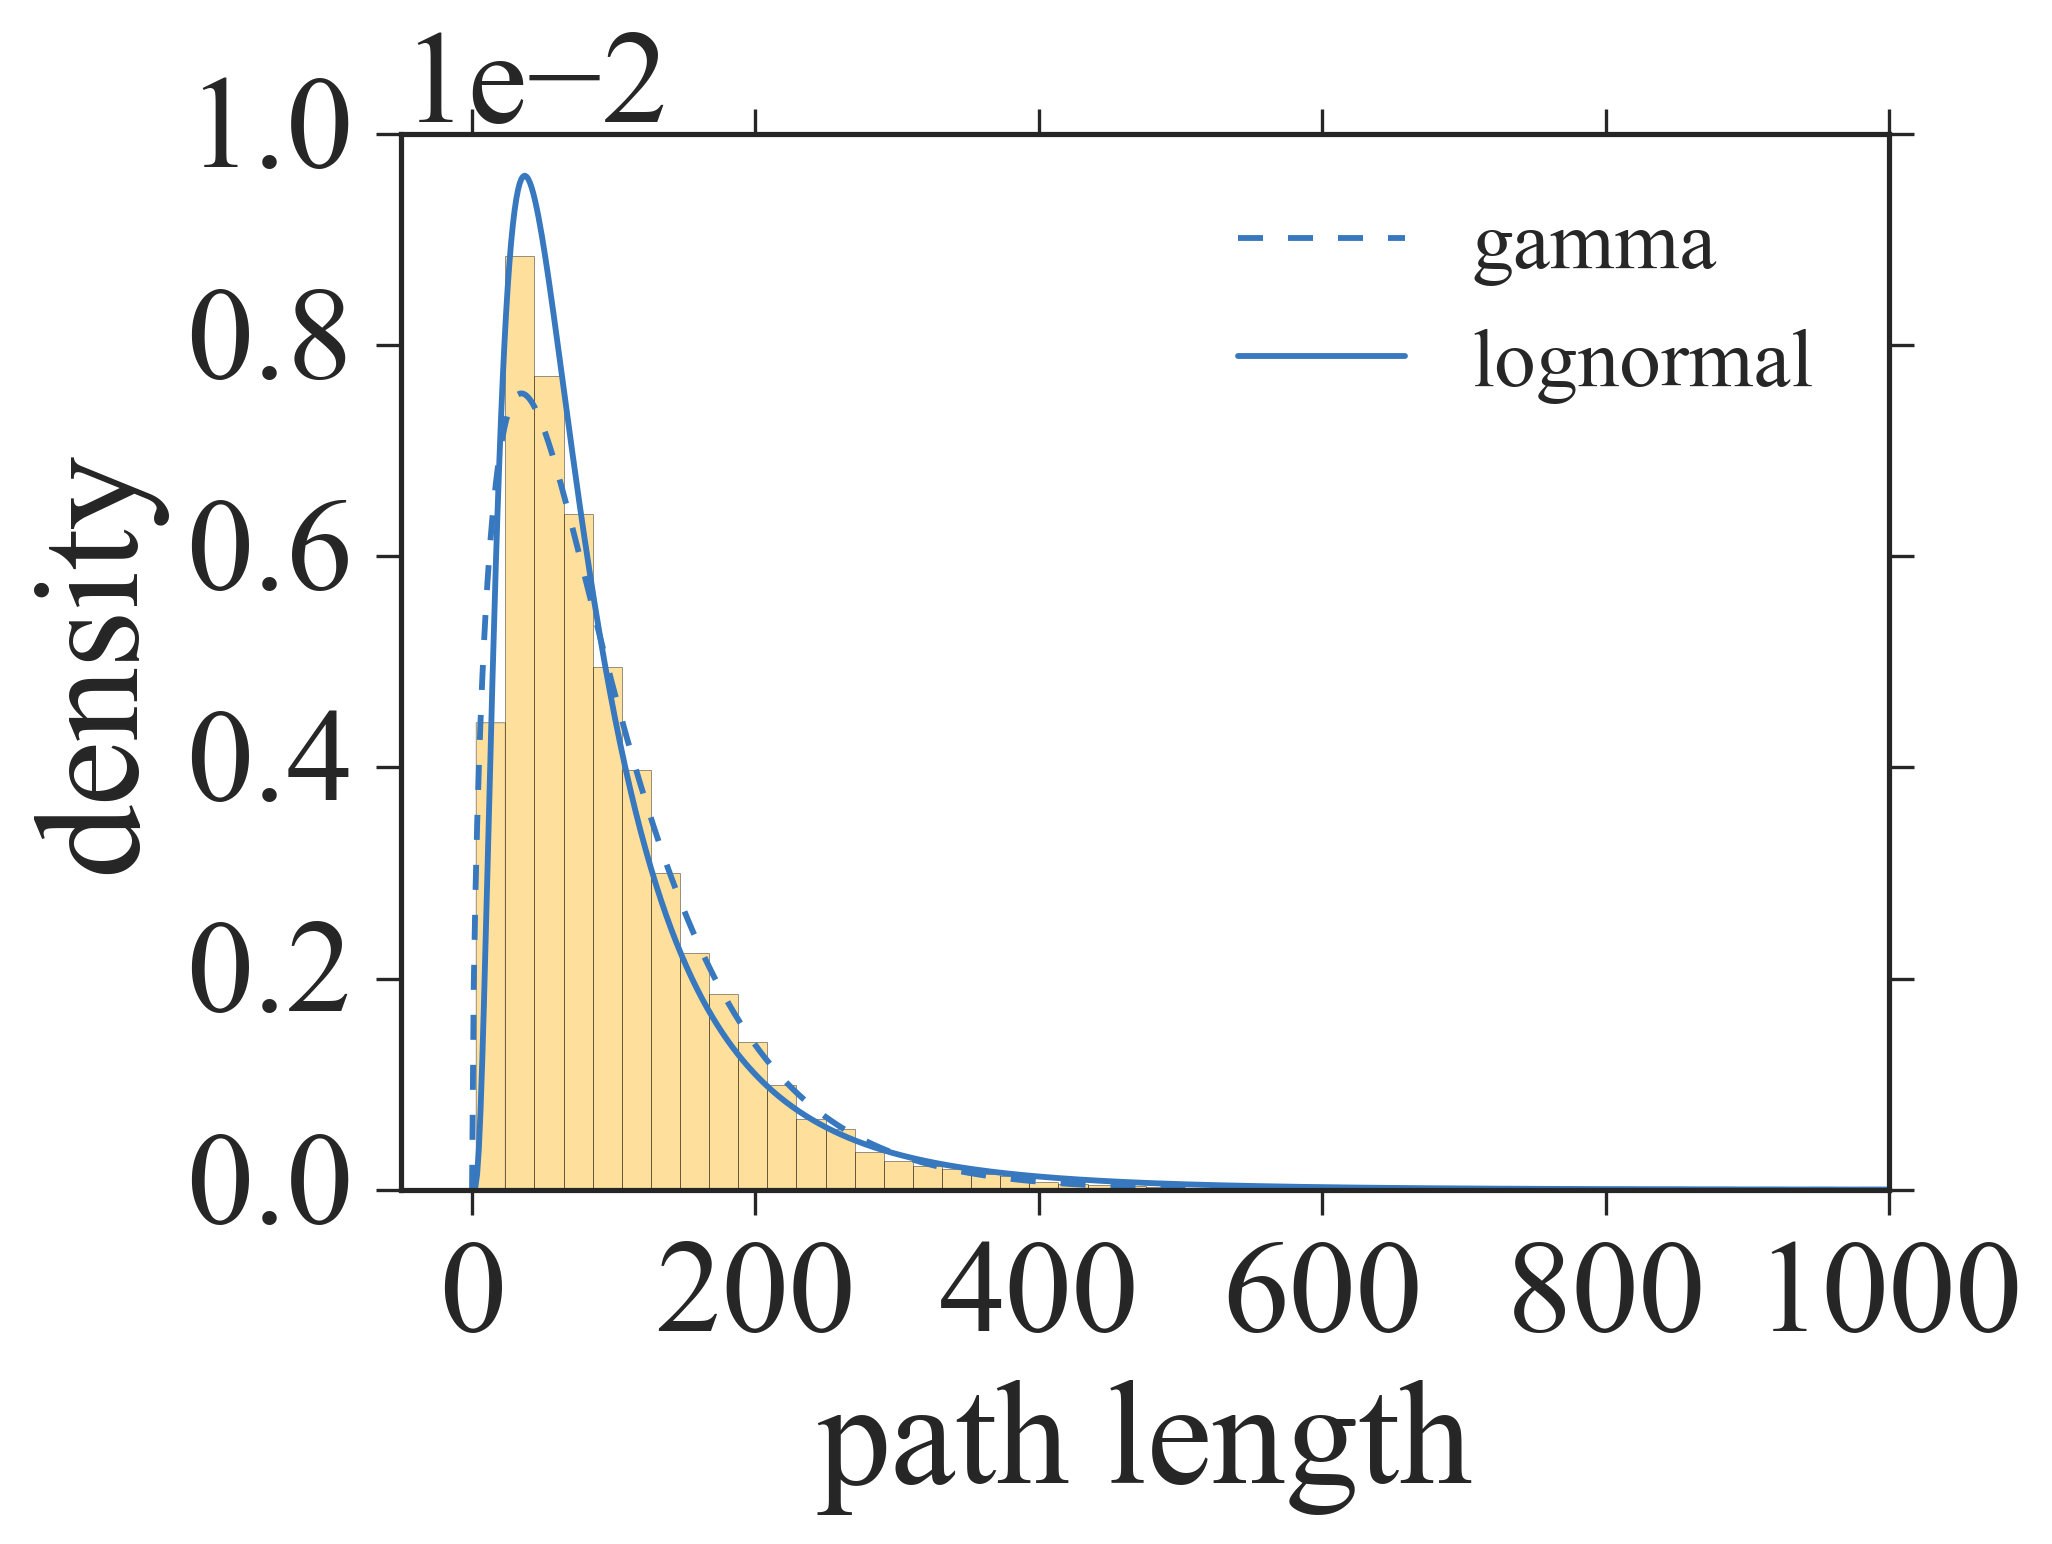
\includegraphics[width=0.45\linewidth,keepaspectratio]{./pics/path_length/path_length_motion22.png}\qquad
			\label{fig:path_lengths_22}}
			\subfloat[][]{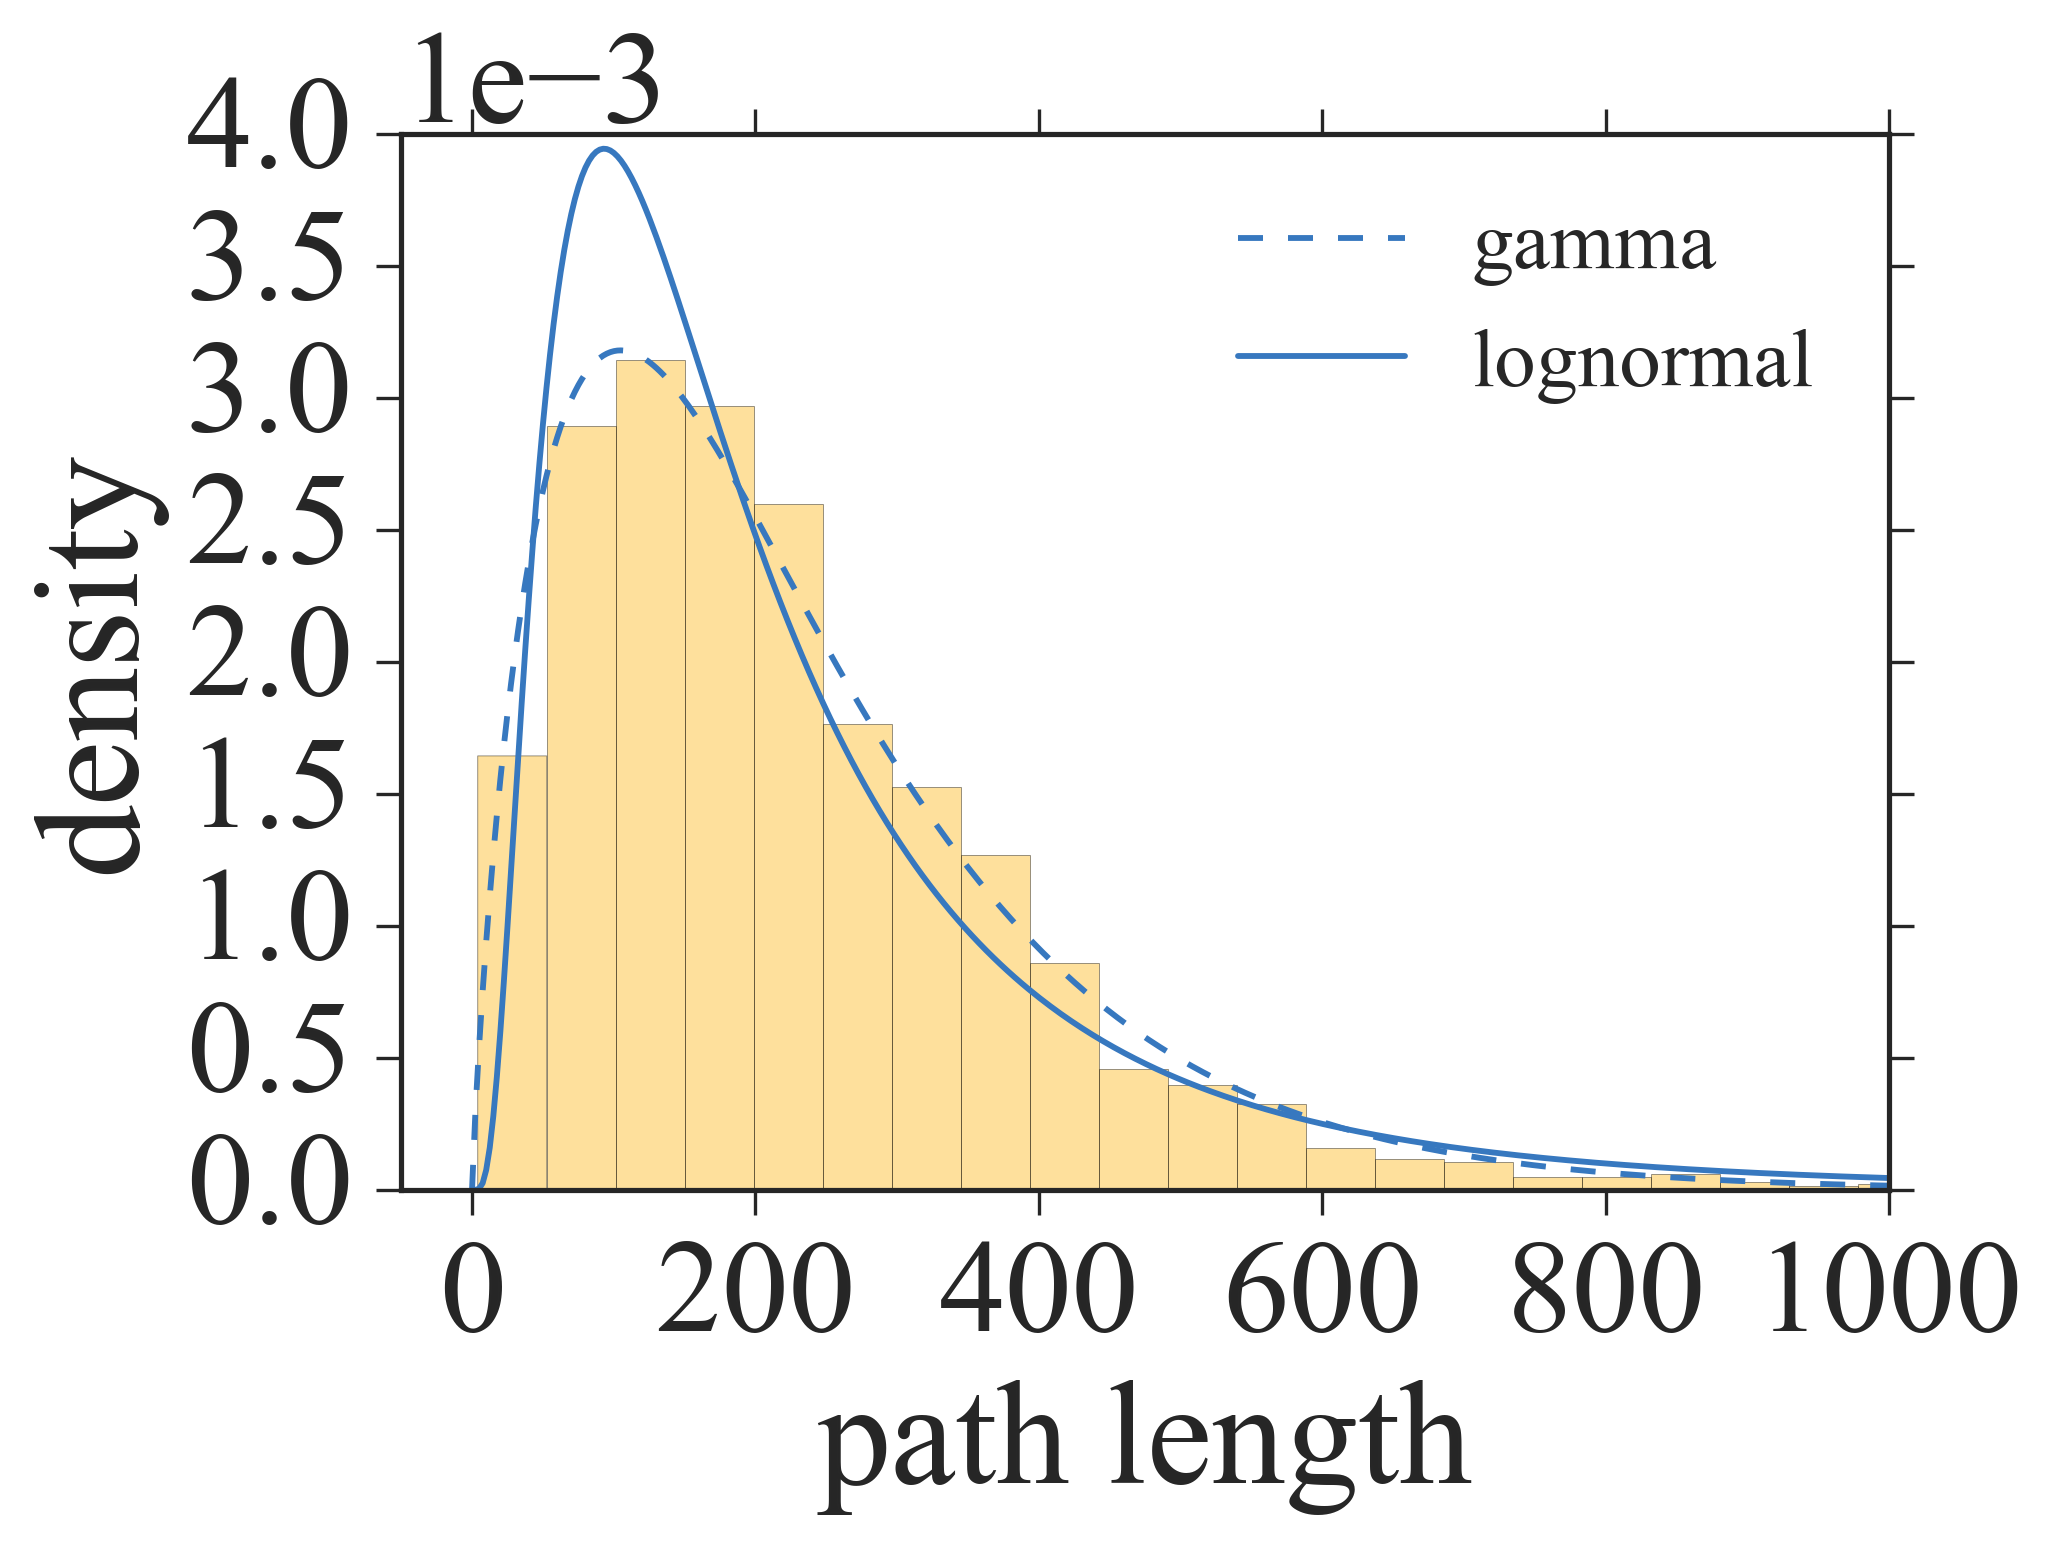
\includegraphics[width=0.45\linewidth,keepaspectratio]{./pics/path_length/path_length_motion35.png}
			\label{fig:path_lengths_35}}

			\caption[Path length distribution]{Path length distributions for \series{22}.}
			\label{fig:path_lengths}
	\end{figure}
\end{frame}

% expected questions:

%How does a prospective algorithm look like? What does it compute? Is it efficient?

\end{document}
                                       
